%\pdfoutput=0
%%%%%%%%%%%%%%%%%%%%%%%%%%%%%%%%%%%%%%%%%%%%%%%%%%%%%%%%%%%%%%%%%%%
%%%%%%%%%%%%%%%%%%%%%%%%%%%%%%%%%%%%%%%%%%%%%%%%%%%%%%%%%%%%%%%%%%
% �bernommen vom EP Skript
%%%%%%%%%%%%%%%%%%%%%%%%%%%%%%%%%%%%%%%%%%%%%%%%%%%%%%%%%%%%%%%%%%
\documentclass[11pt, twoside, a4paper]{book}

\usepackage{graphicx}
\usepackage[utf8]{inputenc}
\usepackage{ngerman}
%\usepackage{lineno}
\usepackage{verbatim}
%\usepackage{comment}
\usepackage[squaren]{SIunits}
\usepackage{amsmath}
\usepackage{amsfonts}
\usepackage{amssymb}
\usepackage{enumitem}
\usepackage{fancyhdr}
\usepackage{textcomp}
\usepackage{subcaption}
%\usepackage{subcaption}
\usepackage[noadjust]{marginnote}
\usepackage{tikz}
%\usepackage{pgfplots}	%Hiermit kann man Plots direkt in LaTex mit tikz Befehlen zeichnen. Erzeugt Kompatibilit�tswarnung. Brauchen wir momentan nicht!
\usepackage{nicefrac}
\usepackage{framed}
\usetikzlibrary{calc,intersections}
\usetikzlibrary{arrows}
\usetikzlibrary{decorations.markings}
\usetikzlibrary{decorations.pathreplacing}
\makeatletter

% Data Flip Flip (DFF) shape
\pgfdeclareshape{dff}{
  % The 'minimum width' and 'minimum height' keys, not the content, determine
  % the size
  \savedanchor\northeast{%
    \pgfmathsetlength\pgf@x{\pgfshapeminwidth}%
    \pgfmathsetlength\pgf@y{\pgfshapeminheight}%
    \pgf@x=0.5\pgf@x
    \pgf@y=0.5\pgf@y
  }
  % This is redundant, but makes some things easier:
  \savedanchor\southwest{%
    \pgfmathsetlength\pgf@x{\pgfshapeminwidth}%
    \pgfmathsetlength\pgf@y{\pgfshapeminheight}%
    \pgf@x=-0.5\pgf@x
    \pgf@y=-0.5\pgf@y
  }
  % Inherit from rectangle
  \inheritanchorborder[from=rectangle]

  % Define same anchor a normal rectangle has
  \anchor{center}{\pgfpointorigin}
  \anchor{north}{\northeast \pgf@x=0pt}
  \anchor{east}{\northeast \pgf@y=0pt}
  \anchor{south}{\southwest \pgf@x=0pt}
  \anchor{west}{\southwest \pgf@y=0pt}
  \anchor{north east}{\northeast}
  \anchor{north west}{\northeast \pgf@x=-\pgf@x}
  \anchor{south west}{\southwest}
  \anchor{south east}{\southwest \pgf@x=-\pgf@x}
  \anchor{text}{
    \pgfpointorigin
    \advance\pgf@x by -.5\wd\pgfnodeparttextbox%
    \advance\pgf@y by -.5\ht\pgfnodeparttextbox%
    \advance\pgf@y by +.5\dp\pgfnodeparttextbox%
  }

  % Define anchors for signal ports
  \anchor{D}{
    \pgf@process{\northeast}%
    \pgf@x=-1\pgf@x%
    \pgf@y=.5\pgf@y%
  }
  \anchor{CLK}{
    \pgf@process{\northeast}%
    \pgf@x=-1\pgf@x%
    \pgf@y=-.5\pgf@y%
  }
  \anchor{Q}{
    \pgf@process{\northeast}%
    \pgf@y=.5\pgf@y%
  }

  % Draw the rectangle box and the port labels
  \backgroundpath{
    % Rectangle box
    \pgfpathrectanglecorners{\southwest}{\northeast}
    \pgf@anchor@dff@CLK
    \pgf@xa=\pgf@x \pgf@ya=\pgf@y
    \pgf@xb=\pgf@x \pgf@yb=\pgf@y
    \pgf@xc=\pgf@x \pgf@yc=\pgf@y
    \pgfmathsetlength\pgf@x{1.6ex} % size depends on font size
    \advance\pgf@ya by \pgf@x
    \advance\pgf@xb by \pgf@x
    \advance\pgf@yc by -\pgf@x
    \pgfpathmoveto{\pgfpoint{\pgf@xa}{\pgf@ya}}
    \pgfpathlineto{\pgfpoint{\pgf@xb}{\pgf@yb}}
    \pgfpathlineto{\pgfpoint{\pgf@xc}{\pgf@yc}}
    \pgfclosepath

    % Draw port labels
    \begingroup
    \pgf@anchor@dff@D
    \pgftext[left,base,at={\pgfpoint{\pgf@x}{\pgf@y}},x=\pgfshapeinnerxsep]{\raisebox{-0.75ex}{D}}

    \pgf@anchor@dff@Q
    \pgftext[right,base,at={\pgfpoint{\pgf@x}{\pgf@y}},x=-\pgfshapeinnerxsep]{\raisebox{-.75ex}{Q}}
    \endgroup
  }
}
% Key to add font macros to the current font
\tikzset{add font/.code={\expandafter\def\expandafter\tikz@textfont\expandafter{\tikz@textfont#1}}} 
\tikzset{every dff node/.style={draw,minimum width=1.5cm,minimum 
  height=1.5cm,thick,inner sep=1mm,outer sep=0pt,cap=round}}

\makeatother

\makeatletter

\pgfdeclareshape{halfadder}{
  % The 'minimum width' and 'minimum height' keys, not the content, determine
  % the size
  \savedanchor\northeast{%
    \pgfmathsetlength\pgf@x{\pgfshapeminwidth}%
    \pgfmathsetlength\pgf@y{\pgfshapeminheight}%
    \pgf@x=0.5\pgf@x
    \pgf@y=0.5\pgf@y
  }
  % This is redundant, but makes some things easier:
  \savedanchor\southwest{%
    \pgfmathsetlength\pgf@x{\pgfshapeminwidth}%
    \pgfmathsetlength\pgf@y{\pgfshapeminheight}%
    \pgf@x=-0.5\pgf@x
    \pgf@y=-0.5\pgf@y
  }
  % Inherit from rectangle
  \inheritanchorborder[from=rectangle]

  % Define same anchor a normal rectangle has
  \anchor{center}{\pgfpointorigin}
  \anchor{north}{\northeast \pgf@x=0pt}
  \anchor{east}{\northeast \pgf@y=0pt}
  \anchor{south}{\southwest \pgf@x=0pt}
  \anchor{west}{\southwest \pgf@y=0pt}
  \anchor{north east}{\northeast}
  \anchor{north west}{\northeast \pgf@x=-\pgf@x}
  \anchor{south west}{\southwest}
  \anchor{south east}{\southwest \pgf@x=-\pgf@x}
  \anchor{text}{
    \pgfpointorigin
    \advance\pgf@x by -.5\wd\pgfnodeparttextbox%
    \advance\pgf@y by -.5\ht\pgfnodeparttextbox%
    \advance\pgf@y by +.5\dp\pgfnodeparttextbox%
  }

  % Define anchors for signal ports
  \anchor{A}{
    \pgf@process{\northeast}%
    \pgf@x=-1\pgf@x%
    \pgf@y=.5\pgf@y%
  }
  \anchor{B}{
    \pgf@process{\northeast}%
    \pgf@x=-1\pgf@x%
    \pgf@y=-.5\pgf@y%
  }
  \anchor{S}{
    \pgf@process{\northeast}%
    \pgf@y=.5\pgf@y%
  }
  \anchor{C}{
    \pgf@process{\northeast}%
    \pgf@y=-0.5\pgf@y%
  }

  % Draw the rectangle box and the port labels
  \backgroundpath{
    % Rectangle box
    \pgfpathrectanglecorners{\southwest}{\northeast}
    % Angle (>) for clock input

    % Draw port labels
    \begingroup
    \pgf@anchor@halfadder@A
    \pgftext[left,base,at={\pgfpoint{\pgf@x}{\pgf@y}},x=\pgfshapeinnerxsep]{\raisebox{-0.75ex}{A}}
    
    \pgf@anchor@halfadder@B
    \pgftext[left,base,at={\pgfpoint{\pgf@x}{\pgf@y}},x=\pgfshapeinnerxsep]{\raisebox{-0.75ex}{B}}


    \pgf@anchor@halfadder@S
    \pgftext[right,base,at={\pgfpoint{\pgf@x}{\pgf@y}},x=-\pgfshapeinnerxsep]{\raisebox{-.75ex}{S}}

    \pgf@anchor@halfadder@C
    \pgftext[right,base,at={\pgfpoint{\pgf@x}{\pgf@y}},x=-\pgfshapeinnerxsep]{\raisebox{-.75ex}{C}}

    \endgroup
  }
}

% Define default style for this node
\tikzset{every halfadder node/.style={draw,minimum width=1.5cm,minimum 
  height=1.5cm,thick,inner sep=1mm,outer sep=0pt,cap=round}}

\makeatother

\makeatletter

\pgfdeclareshape{fulladder}{
  % The 'minimum width' and 'minimum height' keys, not the content, determine
  % the size
  \savedanchor\northeast{%
    \pgfmathsetlength\pgf@x{\pgfshapeminwidth}%
    \pgfmathsetlength\pgf@y{\pgfshapeminheight}%
    \pgf@x=0.5\pgf@x
    \pgf@y=0.5\pgf@y
  }
  % This is redundant, but makes some things easier:
  \savedanchor\southwest{%
    \pgfmathsetlength\pgf@x{\pgfshapeminwidth}%
    \pgfmathsetlength\pgf@y{\pgfshapeminheight}%
    \pgf@x=-0.5\pgf@x
    \pgf@y=-0.5\pgf@y
  }
  % Inherit from rectangle
  \inheritanchorborder[from=rectangle]

  % Define same anchor a normal rectangle has
  \anchor{center}{\pgfpointorigin}
  \anchor{north}{\northeast \pgf@x=0pt}
  \anchor{east}{\northeast \pgf@y=0pt}
  \anchor{south}{\southwest \pgf@x=0pt}
  \anchor{west}{\southwest \pgf@y=0pt}
  \anchor{north east}{\northeast}
  \anchor{north west}{\northeast \pgf@x=-\pgf@x}
  \anchor{south west}{\southwest}
  \anchor{south east}{\southwest \pgf@x=-\pgf@x}
  \anchor{text}{
    \pgfpointorigin
    \advance\pgf@x by -.5\wd\pgfnodeparttextbox%
    \advance\pgf@y by -.5\ht\pgfnodeparttextbox%
    \advance\pgf@y by +.5\dp\pgfnodeparttextbox%
  }

  % Define anchors for signal ports
  \anchor{A}{
    \pgf@process{\northeast}%
    \pgf@x=-1\pgf@x%
    \pgf@y=.66\pgf@y%
  }
  \anchor{B}{
    \pgf@process{\northeast}%
    \pgf@x=-1\pgf@x%
    \pgf@y=0\pgf@y%
  }
  \anchor{Cin}{
    \pgf@process{\northeast}%
    \pgf@x=-1\pgf@x%
    \pgf@y=-.66\pgf@y%
  }
  \anchor{S}{
    \pgf@process{\northeast}%
    \pgf@y=.66\pgf@y%
  }
  \anchor{C}{
    \pgf@process{\northeast}%
    \pgf@y=-.66\pgf@y%
  }

  % Draw the rectangle box and the port labels
  \backgroundpath{
    % Rectangle box
    \pgfpathrectanglecorners{\southwest}{\northeast}
    % Angle (>) for clock input

    % Draw port labels
    \begingroup
    \pgf@anchor@fulladder@A
    \pgftext[left,base,at={\pgfpoint{\pgf@x}{\pgf@y}},x=\pgfshapeinnerxsep]{\raisebox{-0.75ex}{A}}
    
    \pgf@anchor@fulladder@B
    \pgftext[left,base,at={\pgfpoint{\pgf@x}{\pgf@y}},x=\pgfshapeinnerxsep]{\raisebox{-0.75ex}{B}}

    \pgf@anchor@fulladder@Cin
    \pgftext[left,base,at={\pgfpoint{\pgf@x}{\pgf@y}},x=\pgfshapeinnerxsep]{\raisebox{-0.75ex}{$\text C_{\text{in}}$}}


    \pgf@anchor@fulladder@S
    \pgftext[right,base,at={\pgfpoint{\pgf@x}{\pgf@y}},x=-\pgfshapeinnerxsep]{\raisebox{-.75ex}{S}}

    \pgf@anchor@fulladder@C
    \pgftext[right,base,at={\pgfpoint{\pgf@x}{\pgf@y}},x=-\pgfshapeinnerxsep]{\raisebox{-.75ex}{$\text C_{\text{out}}$}}

    \endgroup
  }
}

% Define default style for this node
\tikzset{every fulladder node/.style={draw,minimum width=1.75cm,minimum 
  height=2.25cm,thick,inner sep=1mm,outer sep=0pt,cap=round}}

\makeatother

\newcommand{\dipcase}[5]{
  \def\dipcasewidth{#3}
  \def\dipcasename{#5}
  \pgfmathsetmacro{\dipcasepinshalf}{(#4)/2}
  \pgfmathsetmacro{\dipcasepinheight}{((\dipcasewidth)/3)}
  \pgfmathsetmacro{\dipcaseheight}{((\dipcasepinheight)*\dipcasepinshalf)}
  \def\dipcasepindistance{1cm}
  \draw (#1,#2) coordinate (dipcaseorigin);

  \draw (dipcaseorigin) rectangle ++(\dipcasewidth, -\dipcaseheight) 
    coordinate (dipcaserb);

  \draw (dipcaseorigin) ++(0.5*\dipcasewidth, 0)
    ++(-0.1*\dipcasewidth, 0)
    arc (-180:0:0.1*\dipcasewidth);

  \foreach \pin in {1, ..., \dipcasepinshalf}
  {
    \pgfmathsetmacro{\rpin}{\pin - 1}
    \foreach \xmirr in {1, -1}
    {
      \ifnum\xmirr=1
        \pgfmathtruncatemacro{\pinnumber}{\pin}
        \draw (dipcaseorigin) ++(0, -\rpin * \dipcasepinheight)
          ++(0, -0.5*\dipcasepinheight) coordinate(dipcasepincenter);
      \else
        \pgfmathtruncatemacro{\pinnumber}{\dipcasepinshalf + \pin}
        \draw (dipcaserb) ++(0, \rpin * \dipcasepinheight)
          ++(0, 0.5*\dipcasepinheight) coordinate(dipcasepincenter);
      \fi
      \draw (dipcasepincenter) coordinate (\dipcasename\pinnumber);

      \draw (dipcasepincenter) 
        ++(0, \dipcasepinheight/4) 
        -- ++(-\dipcasepinheight/4*\xmirr, 0)
        -- ++(0, -\dipcasepinheight/2)
        -- ++(\dipcasepinheight/4*\xmirr, 0);

    }
  }
}


\newcommand{\mymeter}[2] 
{  % #1 = name , #2 = rotation angle
\begin{scope}[transform shape,rotate=#2]
\draw[thick] (#1)node(){$\mathbf V$} circle (11pt);
\draw[rotate=45,-latex] (#1)  +(-17pt,0) --+(17pt,0);
\end{scope}
}
\usepackage[european resistors]{circuitikz}
\usepackage[ 
    top=2cm, 
    bottom=2cm, 
    outer=3cm, 
    inner=3cm,
    marginparwidth=2.5cm,
		headheight=14pt
  ]{geometry}

\usepackage{parskip}
\usepackage{pdfpages}
%\usepackage{hyperref}
\usepackage{import}

\setlength{\parindent}{0pt}

\newcommand{\experimentheader}[4]
{
  \iftutor{{\bf Schwierigkeitsgrad:} #1\\}
  \iftutor{{\bf Dauer:} #2\\}
  {\bf Ger\"ate:} #3\\
  {\bf Bauteile:} #4
}

\newcommand{\hintboxNone}{0}
\newcommand{\hintboxExclamation}{1}
\newenvironment{hintbox}[4][\hsize]
{
  \def\FrameCommand
  {%
    {\color{#3}\vrule width 3pt}%
    \hspace{0pt}%must no space.
    \fboxsep=\FrameSep\colorbox{#4}%
  }%
  \MakeFramed{\hsize#1\advance\hsize-\width\FrameRestore}%
  \mbox{\textbf{#2}:}%
}
{
  \endMakeFramed
}
\newcommand{\xhintbox}[3]
{
  \begin{hintbox}{Achtung}{red!50}{red!10}
    #3
  \end{hintbox}
}

\newenvironment{hint}
{
  \begin{hintbox}{Hinweis}{green!50}{green!10}
}
{
  \end{hintbox}
}

\newenvironment{definition}
{
  \begin{hintbox}{Definition\\}{white!50}{white!10}
}
{
  \end{hintbox}
}

\newenvironment{important}
{
  \begin{hintbox}{Hinweis}{gray!50}{gray!10}
}
{
  \end{hintbox}
}

\newenvironment{jason}
{
  \begin{hintbox}{Achtung}{red!50}{red!10}
}
{
  \end{hintbox}
}

\newcommand{\mandatoryenumi}
{
  \renewcommand{\labelenumi}{\arabic{enumi}.} 
}
\newcommand{\optionalenumi}
{
  \renewcommand{\labelenumi}{$\bigstar$\quad\arabic{enumi}.} 
}
\newcommand{\mandatoryenumii}
{
  \renewcommand{\labelenumii}{(\alph{enumii})} 
}
\newcommand{\optionalenumii}
{
  \renewcommand{\labelenumii}{$\bigstar$\quad(\alph{enumii})} 
}
\newcommand{\icname}[1]{\mbox{\tt #1}}


  %\newcommand{\iftutor}[1]{}
\newcommand{\ifnotutor}[1]{#1}

  \newcommand{\iftutor}[1]{#1}
\newcommand{\ifnotutor}[1]{}


\newenvironment{tutorhint}{\comment}{\endcomment}
\newenvironment{todo}{\comment}{\endcomment}
\newenvironment{solution}{\comment}{\endcomment}
\iftutor
{
  \renewenvironment{todo}
  {
    \hintbox{Todo}{red!50!yellow!90}{red!50!yellow!20}
  }
  {
    \endhintbox
  }
  \renewenvironment{tutorhint}
  {
    \hintbox{Tutorenhinweis der Stunde}{blue!50}{blue!10}
  }
  {
    \endhintbox
  }
  \renewenvironment{solution}
  {
    \hintbox{L\"osung}{black!80}{black!5}
  }
  {
    \endhintbox
  }
}
\newcommand{\etutorhint}[1]
{
  \iftutor{
    \tutorhint
      #1
    \endtutorhint
  }
}
\newcommand{\esolution}[1]
{
  \iftutor
  {
    \solution
    #1
    \endsolution
  }
}
\newcommand{\etodo}[1]
{
  \iftutor
  {
    \todo
    #1
    \endtodo
  }
}


%%%%%%%%%%%%%%%%%%%%%%%%%%%%%%%%%%%%%%%%%%%%%%%%%%%%%%%%%%%%%%%%%

 \setcounter{tocdepth}{0}
 \setcounter{totalnumber}{6}
 \setcounter{topnumber}{6}
 \setcounter{bottomnumber}{6}

%%%%%%%%%%%%%%%%%%%%%%%%%%%%%%%%%%%%%%%%%%%%%%%%%%%%%%%%%%%%%%%%%%%

 \newcommand{\Ohm}{$\mathrm\Omega$}
 \newcommand{\sym}[1]{$ #1 $}
 %\newcommand{\degree}{$^{\circ}$} 	%already defined somewhere else...
 \newcommand{\ret}{$[\hookleftarrow]$}
 \newcommand{\bs}{\tt\symbol{'134}}
 \newcommand{\us}{\tt\symbol{95}}

%%%%%%%%%%%%%%%%%%%%%%%%%%%%%%%%%%%%%%%%%%%%%%%%%%%%%%%%%

\hyphenation{ Tor-sions-mo-dul Tor-sions-schwing-ung  Boltz-mann Ab-len-kung Be-schleu-ni-gungs-span-nung}

%\makeindex

\let\person=\textsc
\newcommand{\komplex}[1]{\ensuremath{\mathfrak{#1}}}%

\begin{document}

\frontmatter


\ifnotutor{\title{\Huge Physikalisches Praktikum\\
f"ur Nebenfach Physik}}
\iftutor{\title{\Huge Nebenfach Praktikum\\
Tutorenversion}}

\author{Dr.~Jens Weingarten, Prof.~Dr.~Arnulf Quadt}
%\edition{1}
 
\maketitle
%das Folgende macht das inhaltverzeichnis schoen
\makeatletter
\renewcommand*{\l@chapter}{\@dottedtocline{0}{1.5em}{2.3em}}
\makeatother

\tableofcontents

%
%%%%%%%%%%%%%%%%%%%%%%%%%%%%%%%%%%%%%%%%%%%%%%%%%%%%%%%%%%%%%%%%%%%

\chapter*{Vorwort}

\addcontentsline{toc}{chapter}{Vorwort}


Herzlich Willkommen zum physikalischen Praktikum im Nebenfach an der Universit"at
G"ottingen. Diese Praktikumsanleitung enth"alt alle Informationen, die Sie ben"otigen, um das einsemestrige Praktikum erfolgreich zu absolvieren.
%wird Sie die n"achsten zwei bis drei Semester
%begleiten. Das Grundpraktikum f"ur das Fach Physik
%beinhaltet die Vorlesung \glqq{}Grundlagen des Experimentierens\grqq{} 
%(GdE) sowie 25~Versuche und erstreckt sich "uber zwei Semester. Es
%soll im Regelfall im 2.~und 3.~Semester absolviert werden. Das
%separate Projektpraktikum schlie"st sich im 4.~Semester an.

Das Praktikum (Modul B.Phy-NF.7004) wird ben"otigt f"ur den Bachelor in Chemie, Mathematik, Geologie, Biologie, Bio-Diversit"at, Mineralogie, Physiologie und Molekulare Medizin sowie f"ur den Zwei-Fach Bachelor in Biologie, Chemie, Geowissenschaften und Mathematik. Dieses Praktikum wird mit 4~SWS angerechnet und bringt 4~Credits.
%Physik und f"ur den 2-F"acher-Bachelor (Lehramt an Gymnasien) mit Physik
%als Fach. 
%Dieses Praktikum wird mit 4~SWS angerechnet und bringt 12~Credits -- 2~Credits f"ur
%die GdE als B.phy.410.1 und 10~Credits f"ur die 25~Versuche als
%B.phy.410.2. F"ur den Bachelor in Physik ist zus"atzlich auch
%das Projektpraktikum (Modul B.phy.604) erforderlich.\footnote{Das
%Projektpraktikum kann auch von Lehramtstudentinnen und -studenten
%durchgef"uhrt und als Studienleistung anerkannt werden. Bitte
%informieren Sie sich bei Ihrer Studienberaterin f"ur das
%Lehramt/Zweif"acher-Bachelor.} 


Das G"ottinger Nebenfach-Physikpraktikum f"uhrt anhand ausgew"ahlter, vorgefertigter Versuche
in einen weiten Bereich physikalischer Grundlagen, in den Umgang mit
Apparaturen und Messger"aten und in die Technik des physikalischen
Experimentierens ein und stellt damit einen wesentlichen Teil der
traditionellen Grundausbildung in Physik dar. Ziel ist hierbei auch 
eine Vertiefung des
in der Vorlesung ''Experimentalphysik I im Nebenfach'' erlernten Stoffes durch eigenes Umsetzen
und das Erfahren von Physik (\textit{learning by doing}). Sie erlernen
den Umgang mit verschiedensten Ger"aten und erfahren durch eigenes
Tun, wie eine physikalische Aufgabenstellung experimentell und
methodisch angegangen wird (\textit{hands on physics}). %Problem -
%Analyse - Bearbeitung - L"osung - Dokumentation, dies ist die
%Sequenz, die Sie in Ihrem ganzen "`Physik"=Leben"' begleiten wird.
Hierbei spielt auch Gruppen- oder Teamarbeit eine wichtige Rolle.
Nutzen Sie die Gelegenheit im Praktikum auch dies zu "uben, und
bringen Sie sich aktiv ein. Es wird sich auszahlen.

Dieses Handbuch beschreibt derzeit 20~Versuche, wovon nur 14
verpflichtend durchgef"uhrt werden m"ussen. %Zu Abschnitt 15 (Ferro-, Para-,
%Diamagnetismus) stehen zwei Versuche, zu Abschnitt 17 (Elektronik)
%stehen drei Versuche zur Auswahl, wovon jeweils einer durchgef"uhrt wird.
%Sprechen Sie die Auswahl bitte rechtzeitig mit Ihren Praktikumspartnern und
%Ihrem/r Betreuer/in ab.

%Mit dem seit 2002 eingef"uhrten Projektpraktikum, welches sich an die
%vorgefertigten Versuche anschlie"st, soll verst"arkt auch das
%eigenst"andige wissenschaftliche Arbeiten gef"ordert werden. Hierzu
%werden nur Themen (bzw. Aufgabenstellungen) vorgegeben oder auch von
%den Praktikantinnen und Praktikanten selbst ausgew"ahlt, die dann
%eigenst"andig in der Gruppe (max. 6~Personen) mit
%Hilfestellung eines Betreuers bearbeitet werden. Weitere Einzelheiten zum
%Projektpraktikum sind in diesem Handbuch im Teil \glqq
%Projektpraktikum\grqq{} angef"uhrt.

%Wir legen hiermit ein wiederum "uberarbeitetes Handbuch
%f"ur das G"ottinger Grundpraktikum Physik vor. 
%Wir m"ochten uns
%bei allen Praktikantinnen und Praktikanten, sowie allen Betreuerinnen
%und Betreuern bedanken, die durch ihre Hinweise und Vorschl"age geholfen
%haben, diese Anleitung zu verbessern. Ein besonderer Dank gilt den 
%Beteiligten des Lehrportals, die diese Anleitung mit einer online-Version
%und Videos unterst"utzen und mit verbesserten Abbildungen zu dieser
%Version des Handbuchs beigetragen haben. Trotz der Verbesserungen ist 
%es nur nat"urlich, dass sich auch wieder neue
%Fehler und Unzul"anglichkeiten in dieses Handbuch eingeschlichen haben.
%Wir w"aren dankbar, wenn Sie uns Fehler und auch Verbesserungsvorschl"age
%\emph{sofort} mitteilen w"urden (E-Mail: {\footnotesize
%\url{jgrosse1@uni-goettingen.de}}). Wir werden diese dann
%schnellstm"oglich beheben und auf den Web"=Seiten des Praktikums eine
%verbesserte Version der jeweiligen Anleitung zur Verf"ugung stellen.
%Noch sind nicht alle Versuche und ihre Anleitungen auf dem Stand, den
%Sie und wir gerne h"atten. Dies werden Sie sicherlich feststellen.
%Bedenken Sie, dass diese Anleitung und auch die "Uberarbeitung und
%Erneuerung der Versuche sehr viel Arbeit erfordert, und wir bei der
%derzeitigen Personal- und Betreuungssituation nicht alles umsetzen
%k"onnen, was Sie sich und wir uns w"unschen.

%Wir modernisieren das Grundpraktikum Physik weiterhin
%kontinuierlich durch Neuanschaffungen, Versuchsmodifikationen und
%Entwicklung neuer Versuche. Daneben gibt es Apparaturen, die etwas
%\glqq{}altmodischer\grqq{} aussehen, aber doch noch ganz ihrer
%(didaktischen) Aufgabe gerecht werden. Es kostet gro"se M"uhe, alle
%diese Apparaturen in einem einwandfreien Zustand zu erhalten.
%Sollten Sie dennoch Fehler feststellen, so geben Sie uns bitte
%sofort Bescheid. Nur dann k"onnen wir f"ur Abhilfe sorgen.

%Auch nach dem Druck dieser \glqq{}Praktikumsanleitung\grqq{} werden
%Versuche weiterentwickelt und verbessert, so dass es zu Abweichungen
%des aktuellen Versuches von dieser Anleitung kommen kann. Bedenken
%Sie bitte, dass zwischen Drucklegung und Ihrer Durchf"uhrung des
%Versuches schon eine lange Zeitspanne vergangen sein kann (im
%Extremfall "uber ein Jahr). Wir bem"uhen uns, Ihnen solche "Anderungen
%und Verbesserungen rechtzeitig mitzuteilen, hoffen aber auch, dass
%Sie diese Verbesserungen honorieren werden. Wir werden versuchen,
%auf den Webseiten immer aktuelle Versuchsanleitungen zur Verf"ugung
%zu stellen. Es lohnt sich also bestimmt, von Zeit zu Zeit auf den
%Web-Seiten des Praktikums {\footnotesize
%\url{http://www.praktikum.physik.uni-goettingen.de}} nachzusehen, da
%wir uns bem"uhen werden, dort immer die aktuellsten Informationen zu
%publizieren. Auf den Webseiten finden Sie auch wertvolle Hinweise,
%Kontaktadressen, Termine, Gruppeneinteilungen und eine E-Mail Liste.
%Die E-Mail-Liste ist zur Vermeidung von \acro{SPAM}-Mail 
%nur nach einem Login "uber das Benutzerkonto, welches Sie bei
%der online-Anmeldung angelegt haben, zu erreichen.

In diesem Handbuch finden Sie eine kleine Abhandlung "uber die
Grundlagen der Fehlerrechnung und Protokollerstellung. 
%W"ahrend der
%\glqq Grundlagen des Experimentierens\grqq{} werden Sie davon bereits
%profitiert haben und k"onnen das dort gelernte hier entsprechend anwenden.
%Sprechen Sie
%bitte Ihren Betreuer/Ihre Betreuerin an, damit diese/r an den ersten
%Versuchstagen die Fehlerrechnung und Protokollerstellung nochmal an
%einem konkreten Beispiel mit Ihnen und Ihrer Gruppe "ubt.

Bitte bedenken Sie auch immer, dass Ihre Betreuerinnen und Betreuer
f"ur \emph{Ihr} Praktikum, also f"ur \emph{Ihren} Lernerfolg, viel
Arbeit und Zeit investieren. Dies geschieht neben eigenem Studium
oder eigener Promotion und resultiert in einer Belastung, die weit
"uber das hinausgeht, was als Lehrverpflichtung von Betreuer(innen)
im Durchschnitt an der Fakult"at erbracht wird. Leider
stehen uns nicht so viele Betreuer(innen) zur Verf"ugung, wie wir dies aus
praktischen und didaktischen Erw"agungen f"ur sinnvoll erachten.
Erleichtern Sie deshalb bitte Ihren Betreuerinnen und Betreuern
diese Belastung durch Ihre engagierte, aktive, gut vorbereitete und
m"oglichst eigenst"andige Mitarbeit im Praktikum und
\glqq{}zahlen\grqq{} Sie deren Engagement mit Ihrem pers"onlichen
guten Lernerfolg zur"uck. Nur Ihr \emph{aktives und eigenst"andiges}
Arbeiten erzielt auch eine hohe Nachhaltigkeit des Erlernten und
schafft so das solide Wissensfundament, auf dem Sie Ihre Zukunft
aufbauen k"onnen.

Zusammenfassend w"unschen Ihnen alle Betreuerinnen und Betreuer des
Praktikums viel Spa"s im und einen guten Lernerfolg durch das
Praktikum. Wir alle, insbesondere Ihre Betreuerinnen und Betreuer,
bem"uhen uns, damit dies -- Ihre Mithilfe angenommen -- auch erreicht
werden kann.


%\signature{G"ottingen}{im Oktober 2015}{Dr. Jens Weingarten}



%%%%%%%%%%%%%%%%%%%%%%%%%%%%%%%%%%%%%%%%%%%%%%%%%%%%%%%%%%%%%%%%%%%

%%%%%%%%%%%%%%%%%%%%%%%%%%%%%%%%%%%%%%%%%%%%%%%%%%%%%%%%%%%%%%%%%%%
% JW: Zum kompilieren verwende Ausgabeprofil "LaTex => PDF"
%%%%%%%%%%%%%%%%%%%%%%%%%%%%%%%%%%%%%%%%%%%%%%%%%%%%%%%%%%%%%%%%%%%


\mainmatter

%%%%%% define header and footer style %%%%%%%%%%%%%%%%%%%%
\pagestyle{fancy}
\fancyhead{} % clear all header fields
\fancyhead[RO,LE]{\leftmark} %Kapitelnummer und -�berschrift Header au�en
\fancyfoot{} % clear all footer fields
\fancyfoot[LE,RO]{\thepage}	%Seitenzahl Footer au�en an der Seite
\renewcommand{\headrulewidth}{0.4pt}
\renewcommand{\footrulewidth}{0.4pt}
%%%%%%%%%%%%%%%%%%%%%%%%%%%%%%%%%%%%%%%%%%%%%%%%%%%%%%%%%%%%
%
\part{Vorbemerkungen}

\renewcommand{\thechapter}{\Alph{chapter}}

%%%%%%%%%%%%%%%%%%%%%%%%%%%%%%%%%%%%%%%%%%%%%%%%%%%%%%%%%%%%%%%%%%%

\chapter{Praktikumsordnung} \label{v:ordnung}

Das Physikalische Praktikum für Nebenfach Physik (B.Phy-NF.7004) besteht aus 14 Versuchen, die während der Vorlesungszeit eines Semesters durchgeführt werden. An einem Praktikumstag werden zwei Versuche durchgeführt, die Termine können dem Kursplan entnommen werden, der vor Beginn des Praktikums auf den Webseiten des Physikalischen Praktikums für Nebenfach Physik veröffentlicht wird. \\
\textbf{Versuche aus einem vorherigen Kurs können nicht angerechnet werden.}

Das Praktikum beginnt mit der obligatorischen Einführungsveranstaltung mit Sicherheitsbelehrung. Eine Teilnahme am Praktikum ohne Sicherheitsbelehrung ist nicht möglich. Sollte das Praktikum zum wiederholten Male belegt werden, ist die Einführungsveranstaltung erneut zu besuchen.

%**********************************************************************************************************************
%**********************************************************************************************************************

%\section{Ablauf des Praktikums}
%
%\begin{enumerate}
	%%
	%\item Das Praktikum erstreckt sich über ein Semester. Wird das Praktikum nicht in diesem Semester abgeschlossen, so muss es erneut belegt werden. Versuche aus dem vorherigen Kurs können nicht angerechnet werden.
	%%
	%\item Das Praktikum umfasst 14 Versuche. Die Termine können dem Kursplan entnommen werden, der vor Beginn des Praktikums auf den Webseiten des Physikalischen Praktikums für Nebenfach Physik veröffentlicht wird.
	%%
	%\item Wenn ein Versuch nicht testiert wurde, 
	%%
	%\item Das Praktikum beginnt mit der obligatorischen Einführungsveranstaltung mit Sicherheitsbelehrung. Eine Teilnahme am Praktikum ohne Sicherheitsbelehrung ist nicht möglich. Sollte das Praktikum zum wiederholten Male belegt werden, ist die Einführungsveranstaltung erneut zu besuchen.
	%%
	%\item Mit der Anmeldung zum Praktikum verpflichtet sich der/die Praktikant/in zur regelmäßigen Teilnahme.
%\end{enumerate}

%**********************************************************************************************************************
%**********************************************************************************************************************


%Es hat Vorteile, wenn eine Zweiergruppe alle Versuch des Praktikums gemeinsam durchf"uhrt. Da dies aufgrund terminlicher Bedingungen nicht immer m"oglich ist, ist es jedoch nicht zwingend.\\
%An jedem Arbeitstag werden von jeder Arbeitsgruppe je 2 Versuche durchgef"uhrt. Nach der Vorbesprechung w"ahlen die Zweiergruppen sich ihre 14 Versuche (7 Arbeitstage) aus den m"oglichen Terminen aus. Es m"ussen aus den Bereichen Mechanik (Versuche 1-10) und Elektrik (Versuche 11-20) jeweils mindestens 6 Versuche ausgesucht werden.

%\noindent
%Es gelten folgende organisatorische Regeln\index{Regeln} f"ur das Praktikum, die einen reibungslosen und effektiven Ablauf des Praktikums erm"oglichen sollen. Diese sind immer zu beachten.

\section{Voraussetzungen zur Teilnahme}

Voraussetzungen zur Teilnahme am Nebenfachpraktikum Physik sind die erfolgreiche Teilnahme an der Vorlesung "`Experimentalphysik I im Nebenfach"' (B.Phy-NF.7001 oder B.Phy-NF.7002), als auch die persönliche Teilnahme an der Einführungsveranstaltung des Praktikums. 

\section{Anmeldung und Gruppeneinteilung}

Zur Teilnahme am Praktikum melden Sie sich bitte auf StudIP für die Veranstaltung an.\\
Das Praktikum wird in festen Gruppen von bis zu 10 Studierenden durchgeführt. Bitte tragen Sie sich bei der Anmeldung gleich in eine der vordefinierten Gruppen ein.\\
Die Versuche werden in Zweiergruppen durchgeführt, welche zusammen ein Protokoll abgeben. Sollte eine/r der Teilnehmer/innen zur Versuchsdurchführung nicht erscheinen, so kann in Absprache mit dem Betreuer eine Dreiergruppe gebildet werden.

\section{Termine}

Der Termin für die Einführungsveranstaltung wird rechtzeitig in UniVZ und auf StudIP angekündigt. Typischerweise findet diese in der ersten Vorlesungswoche statt.

Die Versuche werden jeweils Mittwoch oder Freitag an 14~Uhr~c.t. durchgeführt. Ab etwa 13:30~Uhr sind die Tutoren in den Praktikumsräumen anzutreffen, damit Sie Ihre Protokolle abgeben oder den Versuch testiert bekommen können. 

\section{Versuchsvorbereitung}

Jede Praktikantin und jeder Praktikant muss sich genügend auf den durchzuführenden Versuch\index{Versuchsvorbereitung} vorbereiten. Die Durcharbeitung der Anleitung zum Praktikum und das Literaturstudium sind obligatorisch. \\
Der schriftliche Kurztest vor Versuchsbeginn (''Quicky'') dient dem Nachweis genügender fachlicher Grundkenntnisse und ausreichender Vorbereitung der Teilnehmer, er bildet die Grundlage für die Teilnahme an den Praktikumsversuchen.

Wer unvorbereitet zu einem Versuch kommt, riskiert, dass er/sie den Versuch an diesem Tag nicht durchf"uhren darf und einen Nachholtermin in Anspruch nehmen muss. Zur Hilfe bei der Vorbereitung sind in der jeweiligen Versuchsanleitung einige Fragen gestellt. 
In der ersten Stunde jeden Praktikumtages prüft der Assistent, ob Sie sich auf die beiden Versuche vorbereitet haben. Dazu k"onnen Sie in den ersten 30 Minuten Fragen zu möglichen Unklarheiten im Versuch an den Assistenten stellen. Anschließend werden Zettel ausgeteilt, auf denen jeweils auf einer Viertelseite 2 der Vorbereitungsfragen schriftlich beantwortetet werden müssen (Quickie). Die Zettel werden sofort durchgesehen und bleiben bei den Assistenten.\\ 
\textbf{Wer beide Fragen falsch beantwortet, wird vom Versuch ausgeschlossen.} Nur eine falsche Antwort führt nicht zum Ausschluss, wohl aber, wenn es schon das zweite Mal ist. 

%Die Betreuerinnen und Betreuer sind gehalten, vor jedem Versuch
%nochmals die Sicherheitsaspekte zum Versuch zu erl"autern und deren
%Verst"andnis zu "uberpr"ufen.

\section{Durchführung}

\textbf{Die Versuchsdurchführung beginnt um 14~Uhr~c.t. Erheblich verspätetes Erscheinen führt zum Ausschluss an der Durchführung des Versuchs.}\\
Vor dem Beginn der Messungen mache man sich mit den Apparaturen vertraut, d.h. wie sind welche Messgeräte anzuschließen, wie funktionieren sie, wie werden sie abgelesen, welche Fehler haben sie, bei welchen Apparaturen ist besondere Vorsicht geboten, usw. Insbesondere bei elektrischen Stromkreisen ist darauf zu achten, dass Strom und
Spannungen sehr gefährlich sein können! Messgeräte sind vor dem Gebrauch - sofern möglich - auf Funktionsfähigkeit zu testen und auf den richtigen Messbereich einzustellen. Manchmal ist es hilfreich, Schalter und Messgeräte durch Zettel oder ähnliches (z.B. "`Post-it"') zu beschriften, um Irrtümer zu vermeiden. Bei elektrischen Schaltungen ist nach dem Aufbau zunächst der Assistent zu benachrichtigen, erst mit dessen Zustimmung wird die Stromversorgung eingeschaltet! Messkurven sind während der Versuchsdurchführung grafisch darzustellen (Millimeterpapier nicht vergessen!). Jeder ist selbst dafür verantwortlich, dass alle benötigten Daten richtig und vollständig gemessen werden. Bitte denken Sie nach, ob die gemessenen Werte sinnvoll sind!

\textbf{Während der Versuchsdurchführung ist ein Messprotokoll\index{Messprotokoll} \emph{dokumentenecht} anzufertigen.} \\
Es darf also nur Kugelschreiber oder Tusche verwendet werden (kein Bleistift). Es wird nichts radiert, sondern nur gestrichen. Datum und Mitarbeiter angeben, Seiten nummerieren. Die Versuchsdurchführung muss nachvollziehbar sein. \\
Darauf müssen folgende Informationen zu finden sein:
\begin{itemize}
	\item Name des Versuchs
	\item Datum der Durchführung 
	\item Namen aller beteiligten Praktikanten 
	\item die gemessenen Werte mit Fehlerangabe.
\end{itemize} 
Das Protokoll muss leserlich sein und sollte übersichtlich gestaltet sein, z.B. durch einleitende Sätze, was mit den dann folgenden Messwerten bestimmt werden soll. Jeder Messwert muss eindeutig mit der gemessenen Größe in Verbindung gebracht werden können, ggf. sollten Skizzen angefertigt werden. Es müssen die tatsächlich gemessenen (direkt abgelesenen) Werte aufgeschrieben werden, zusätzlich ausgerechnete Werte (z.B. Differenzen) dürfen nur zusätzlich aufgeschrieben werden. Dies soll (Kopf-)Rechen- und Denkfehlern
vorbeugen. Zu jedem Messwert ist die Einheit zu notieren! Zu jedem Messwert ist ein Fehler zu notieren (Ablesefehler, Gerätefehler, Schwankungen).

\textbf{Am Ende des Versuchs wird das Messprotokoll vom Assistenten testiert, ansonsten ist es ungültig!}

Sinnigerweise sollte der Versuch erst hiernach abgebaut werden, da u.U. bestimmte Dinge erneut gemessen werden m"ussen oder Daten fehlen.\\ 
{\bf Jede(r) Student/in sollte ein eigenes testiertes Messprotokoll haben.}\\
Erst nachdem der/die Betreuer/in die Werte kontrolliert, das Versuchsprotokoll testiert (Versuchs"=Testat) \index{Versuchs-Testat} und dies in die Karteikarte eingetragen hat,
ist der Versuch abzubauen und alles aufzuräumen. Weiterhin erteilt der Assistent nach Abschluss eines Versuches auch auf der Karteikarte durch Unterschrift ein Vortestat. Dieses dient gleichzeitig als Teilnahme-Beweis.

Nach Beendigung eines Versuchstages\index{Versuchsende}\index{Aufräumen} sind alle Versuche, Geräte und Räume wieder in den ursprünglichen Zustand zu versetzen. Messgeräte, Kabel und Stoppuhren sind wieder an die vorgesehenen Stellen zu bringen. \textbf{Defekte sind sofort einem/r Betreuer/in zu melden.} Flaschen und sonstige Abfälle sind bitte zu entsorgen.


\section{Protokolle}

%Beachten Sie zum Protokoll auch die Hinweise in
%Kapitel~\ref{c:protokoll}. 
Im Protokollkopf müssen der Name des Versuchs und das Datum der Durchführung stehen. Bei einem in Eigenarbeit geschriebenen Protokoll\index{Protokoll} steht als "`Praktikant"' der Name des Praktikanten und unter "`Mitarbeiter"' die Namen der übrigen an der Versuchsdurchführung beteiligten Personen. Bitte auch den Namen des/der Betreuers/in und die eigene E-Mail Adresse im Kopf angeben. 
%Jeder
%Praktikant braucht f"ur die Unterschrift auf der Karteikarte ein
%eigenes Protokoll, welches auch unterschrieben werden
%soll. 

Das Protokoll muss leserlich und übersichtlich gestaltet sein. Es ist für sich eigenständig, also keine Verweise auf die Praktikumsanleitung.\footnote{Sätze wie "`Versuchsdurchführung s. Praktikumsanleitung"' sind überflüssig.} Aus dem Protokoll alleine muss klar verständlich sein, was das Ziel des Versuchs war, wie Sie den Versuch durchgeführt haben und was das Ergebnis des Versuchs ist. Es muss aus dem Protokoll ersichtlich sein, wie die Auswertung aufgebaut ist, d.h. welche Werte gemessen wurden und was man aus diesen Messwerten bestimmen möchte.

Im eigentlichen Teil der Auswertung sind deutlich und nachvollziehbar die einzelnen Auswertungsschritte aufzuschreiben. Einleitende Sätze, was gemessen wurde, und was daraus berechnet wird, sind obligatorisch. Ergebnisse sind deutlich zu kennzeichnen (Rahmen, farbiges Markieren, größere Schrift, usw.). Was sind Zwischen- oder Hilfsergebnisse, was sind Endergebnisse? Alle benutzten Formeln müssen beschrieben sein bzw. deren Herleitung klar werden. Es ist auf eine durchgehend eindeutige Variablendefinition und Variablenbenutzung im Protokoll zu achten. Alle Variablen in den Funktionen sind zu benennen bzw. zu definieren. Die Fehlerrechnung muss nachvollziehbar beschrieben werden (einfacher Mittelwert oder gewichtetes Mittel, ggf. Formel der Fehlerfortpflanzung angeben). Fehler sind sinnvoll anzugeben! Alle Werte haben Einheiten, alle Grafen eine Beschriftung! Bei Vergleich mit Literaturwerten: Woher kommen die Werte (Quellenangabe)? Eine Diskussion der Ergebnisse und der Fehler ist obligatorisch. Dazu muss man sich natürlich vorher die Frage stellen, ob das, was man berechnet hat, ein sinnvolles Ergebnis ist.

Bei der Abgabe des Protokolls muss das dazugehörige original unterschriebene Messprotokoll mit abgegeben werden. Protokolle müssen in geeigneter Form zusammengeheftet sein (einfache Mappe oder Heftung reichen vollkommen), lose Blätter werden nicht akzeptiert.\\
\textbf{Wird ein/e Praktikant/in auf die Auswertung seines/ihres eigenen Protokolls angesprochen und kann keine Auskunft zu den gemachten Rechnungen geben, so gilt das Protokoll als nicht selbständig erstellt und wird nicht testiert.} \\
Protokolle mit einer Auswertung, die nicht auf den eigenen Messdaten basieren, bei denen die Messdaten nachträglich geändert wurden oder bei denen die Liste der am Versuch beteiligten Personen erweitert wurde, gelten als Täuschungsversuch/Urkundenfälschung und werden entsprechend geahndet.
%
%\begin{definition}[Abgabefrist der Protokolle]
% Die Abgabefrist f"ur ein Protokoll betr"agt 2~Wochen nach Durchf"uhrung
% des Versuchs.
%\end{definition}
%

{\bf Ein vollständiges Protokoll muss zum nächsten Praktikumstermin, also innerhalb einer Woche nach der Versuchsdurchführung, abgegeben werden.} 
%Wird das Protokoll {\bf nicht innerhalb von 2~Wochen} abgegeben, {\bf verf"allt das Vortestat und der Versuch muss wiederholt werden.} 

Ein Protokoll gilt nur dann als vollständig, wenn es oben genannte Bedingungen erfüllt. Insbesondere gilt es als nicht vollständig, wenn es außer dem Endergebnis keine Zwischenergebnisse enthält, die den Rechenweg und die Werte nachvollziehbar machen. Sollte das Protokoll für Korrekturen ohne Testat zurückgegeben werden, so gilt erneut die 1~Wochen-Frist ab dem Tag der Rückgabe. Die Korrekturen sind (z.B. als Anhang) zusammen mit dem vollständigen ursprünglichen Protokoll abzugeben. Sie haben die Möglichkeit, jedes Protokoll genau einmal zu überarbeiten. Wird das Protokoll nach der Korrektur immer noch nicht testiert wird, so gilt der Versuch als nicht bestanden und es muss ein Versuch (nicht notwendigerweise derselbe) nachgeholt werden.

Auch für die Rückgabe der Protokolle durch die Assistenten soll die 1-Wochen-Frist eingehalten werden. Das bedeutet, dass nach spätestens vier Wochen feststeht, ob der Versuch testiert wird, oder nicht.

Es ist zu beachten, dass es für jedes Semester einen Termin gibt, ab dem alle bis zu diesem Tag nicht testierten Protokolle nicht mehr angenommen und testiert werden. Dies ist in der Regel der 30.04. für das vergangene Wintersemester und der 31.10. für das vergangene Sommersemester. Dies ist erforderlich, da auch die Betreuer Fluktuationen
unterworfen sind und so der/die Betreuer/in später eventuell Göttingen schon verlassen hat.

\section{Nachholtermine}

\textbf{Es stehen genau zwei Nachholtermine\index{Nachholtermin} für versäumte oder nicht testierte Versuche zur Verfügung.} Sollten Sie aus triftigen Gründen (schwere Erkrankung, o.Ä.) mehr als zwei Versuche versäumen, melden Sie sich bitte umgehend bei der Praktikumsleitung. \textbf{Wenn aus anderen Gründen mehr als zwei Versuche nicht durchgeführt oder testiert werden, gilt das Praktikum als nicht bestanden.}\\
Bitte sorgen Sie dafür, dass ggf. ein/e Partner/in für die Durchführung des Nachholversuchs zur Verfügung steht. Die Nachholtermine finden in den beiden Wochen nach Ende der regulären Versuche statt.
%Um einen Nachholtermin zu bekommen, melden Sie sich bitte z"ugig beim Praktikumsleiter. Es kann vorkommen, dass ein Nachholtermin erst im n"achsten Semster m"oglich ist.


\section{Karteikarte}

Während der Vorbesprechung zum Praktikum werden die Karteikarten\index{Karteikarte} ausgeteilt, die die Praktikantin oder der Praktikant bis zum Abschluss des Praktikums behält. Auf dieser werden dann die Versuchs-Durchführung und Protokoll-Testate vom Assistenten eingetragen und mit Unterschrift bestätigt. Diese Karteikarte ist der Nachweis für die
Gesamtleistung im Praktikum und damit Zulassung zum Noteneintrag in FlexNow, also bitte nicht verlieren.

Nach Abschluss des Praktikums geben Sie bitte Ihre vollständig ausgefüllte Karteikarte bei der Praktikumsleitung ab.


\section{Leistungsnachweis}

Die Gesamtleistung besteht aus 14 durchgeführten und komplett testierten Versuchen. \\
Das Praktikum ist unbenotet und wird nur mit Bestanden oder Nicht Bestanden in FlexNow eingetragen. In besonderen Fällen kann auch ein Schein ausgestellt werden.

%
%%%%%%%%%%%%%%%%%%%%%%%%%%%%%%%%%%%%%%%%%%%%%%%%%%%%%%%%%%%%%%%%%%%

\chapter{Literatur f"ur das Praktikum}

%%%%%%%%%%%%%%%%%%%%%%%%%%%%%%%%%%%%%%%%%%%%%%%%%%%%%%%%%%%%%%%%%%%

Angesichts der sehr unterschiedlichen Vorkenntnisse in Physik und der gro{\ss}en Auswahl physikalischer Lehrb"ucher ist es leider nicht m"oglich, einen einzigen Text als verbindlich zu erkl"aren. Zu Beginn jeder Versuchsanleitung finden Sie eine kurze Einf"uhrung in die zugrundeliegende Physik, welche allerdings keine vollst"andige Darstellung der physikalischen Zusammenh"ange sein kann. Bitte eignen Sie sich daher selbst"andig die zugeh"orige Physik durch Nachlesen in mehreren B"uchern (zur Not auch in Vorg"angerprotokollen\index{Vorg"angerprotokolle}, aber auf Richtigkeit achten!) tiefgehender an. Die unterschiedlichen Darstellungsweisen f"ordern das Verst"andnis. Die nachfolgend  aufgef"uhrten Literaturhinweise sollen dazu  dienen, Ihnen die Suche nach weiterf"uhrendem Material zu erleichtern. Die Aufz"ahlung erhebt weder einen Anspruch auf Vollst"andigkeit, noch stellt sie eine Wertung dar. Die meisten B"ucher sind in der Bereichsbibliothek Physik \textsc{BBP} ausleih- oder einsehbar. Es ist nicht wichtig, von jedem Buch unbedingt die letzte Auflage zu bekommen, da die Physik, die im Praktikum behandelt wird, sich in den letzten 100 Jahren nicht mehr ver"andert hat!

\noindent
Wir empfehlen  Ihnen, die Textstellen nicht isoliert herauszugreifen (Physiklexika sind f"ur die meisten Anf"anger erfahrungsgem"ass nicht  brauchbar!),  sondern Zusammenh"ange herzustellen.   \\
Auch Wikipedia kann nur Anhaltspunkte liefern...


%Als begleitende Literatur\index{Literatur} f"ur das Physikalische
%Praktikum sind prinzipiell alle Physikb"ucher geeignet. Insbesondere
%sind die folgenden B"ucher\index{B"ucher} zu nennen. Die Aufz"ahlung
%erhebt weder einen Anspruch auf Vollst"andigkeit, noch stellt sie
%eine Wertung dar. Welches Buch f"ur Sie pers"onlich das Beste ist,
%k"onnen nur Sie selbst entscheiden. Schauen Sie sich die B"ucher an,
%vergleichen Sie dabei beispielsweise direkt die unterschiedlichen
%Darstellungen eines bestimmten engen Gebietes. W"ahlen Sie dann
%dasjenige Buch aus, welches Ihnen am besten liegt. Neben dieser
%Aufz"ahlung finden sich diese und weitere B"ucher auch im
%Literaturverzeichnis wieder. Die Abk"urzungen der B"ucher werden zum
%Teil auch bei den Versuchen zur Angabe vertiefender Literatur
%benutzt.

%W"ahlen Sie anhand der Sachverzeichnisse\index{Sachverzeichnis} und
%der Stichworte\index{Stichworte} in den Anleitungen die geeignete
%Literatur zum jeweiligen Versuch aus. Zu einigen Versuchen wird
%spezielle Literatur angegeben. Die meisten B"ucher sind in der
%Bereichsbibliothek Physik \acro{BBP} ausleih- oder einsehbar. Wir
%sind bem"uht, die wichtigsten physikalischen Grundlagen in diese
%Anleitung aufzunehmen. Dies kann aber keine vollst"andige Darstellung der den Versuchen zugrunde liegenden Physik sein. 
%Bitte eignen Sie sich daher selbst"andig die zugeh"orige Physik
%durch Nachlesen in mehreren B"uchern (zur Not auch in
%Vorg"angerprotokollen\index{Vorg"angerprotokolle}, aber auf
%Richtigkeit achten!) tiefgehender an. Die unterschiedlichen
%Darstellungsweisen f"ordern das Verst"andnis.


\section{Spezielle Praktikumsb"ucher}

Tabelle~\ref{t:litprakt} enth"alt eine Aufz"ahlung von B"uchern, die
speziell f"ur Physikalische Praktika gedacht sind
(Praktikumsb"ucher\index{B"ucher!Praktikumsb"ucher}) und somit auch
Methodisches und Handlungshinweise enthalten.
%
\begin{table}[h!]
  \centering
  \caption[Praktikumsb"ucher]{\label{t:litprakt}Dedizierte Praktikumsb"ucher}
  \begin{tabular}{lp{11cm}}
    \hline
    K"urzel & Autor, Titel, Verlag, Jahr, Referenz \\
    \hline
    NPP & \person{Eichler, Kronfeld, Sahm}, Das Neue Physikalische Grundpraktikum, Springer, 2001 \\
    Wal & \person{Walcher}, Praktikum der Physik, Teubner, 2004 \\
    Wes & \person{Westphal}, Praktikum der Physik, Springer, 1984 (vergriffen)  \\
    SK & \person{Stuart, Klages}, Kurzes Lehrbuch der Physik, 2009\\
%    Geschke & \person{Geschke}, Physikalisches Praktikum, Teubner, 2001  \cite{geschke} \\
%    BeJo & \person{Becker, Jodl}, Physikalisches Praktikum, VDI-Verlag, 1983 \cite{bejo} \\
%    CIP & \person{Diemer, Basel, Jodl}, Computer im Praktikum  Springer, 1999 \cite{cip} \\
%    Paus & \person{Paus}, Physik in Experimenten und Beispielen,Hanser \cite{paus} \\
    \hline
  \end{tabular}
\end{table}



\section{Allgemeine Physikb"ucher}

Folgende, in Tabelle~\ref{t:litallg} aufgef"uhrte, allgemeine
Physikb"ucher\index{B"ucher!Allgemeine Physik} sind f"ur das
Praktikum und das Studium insgesamt n"utzlich.
%
\begin{table}[h!]
  \centering
  \caption[Allgemeine Physikb"ucher]{\label{t:litallg}Allgemeine Physikb"ucher, die f"ur das Praktikum n"utzlich sind.}
  \begin{tabular}{lp{11cm}}
    \hline
    K"urzel & Autor, Titel, Verlag, Jahr, Referenz \\
    \hline
 BS 1-8 & \person{Bergmann-Schaefer}, Experimentalphysik 1-8, DeGruyter, 2000 \\
 Dem 1-4 & \person{W. Demtr"oder}, Experimentalphysik 1-4, Springer, 2002\\
 Gerthsen & \person{Meschede, Vogel, Gerthsen}, Gerthsen: Physik, Springer, 2003\\
% Halliday & \person{Halliday}, Physik, Springer, 2003 \cite{halli}\\
% Feyn & \person{Feynman} Physics Lectures \cite{feyn1,feyn2,feyn3}\\
% Kohlr 1-3 & \person{Kohlrausch}, Praktische Physik 1-3, Teubner, 2002 \cite{kohlr1,kohlr2,kohlr3} \\
% Wesp & \person{Westphal}, Physik, Springer  \cite{wesp} \\
% Pohl & \person{L"uders-Pohl}, Pohls Einf"uhrung in die Physik, Springer 2004 \cite{pohl}\\
 %Grim 1-4 & \person{Grimsehl}, Lehrbuch der Physik 1-4, Teubner \cite{grim1,grim2,grim3,grim4}\\
% Alonso & \person{Alonso, Finn}, Physik, Oldenbourg, 2000 \cite{alonso} \\
% L"usch 1-3 & \person{L"uscher}, Experimentalphysik 1-3, Piper \cite{luesch1,luesch2,luesch3} \\
% St"ocker & \person{St"ocker}, Taschenbuch der Physik, Harri Deutsch \cite{tabphys} \\
 Tipler & \person{Tipler}, Physik, Spektrum, 1994\\
 Kuhn & \person{Kuhn}, Physik 2, Westermann, 2000\\
 Dorn & \person{Dorn, Bader}, Physik Grundkursband 12/13, Hermann Schroedel Verlag, 1976\\
 Harten & \person{Harten}, Physik f"ur Mediziner: Eine Einf"uhrung, Springer, 2011\\
 Metzler & \person{Grehn, Krause}, Metzler Physik, Schroedel, 2007\\
 \hline
  \end{tabular}
\end{table}


\section{Handb"ucher und Nachschlagewerke}

N"utzliche Hinweise zur Auswertung und Fehlerrechnung, sowie eine Vielzahl von Werten und Materialdaten, findet man in den in Tabelle~\ref{t:litnach} aufgef"uhrten\index{B"ucher!Handb"ucher}
Nachschlagewerken\index{B"ucher!Nachschlagewerke}.
%
\begin{table}[h!]
  \centering
  \caption[Handb"ucher und Nachschlagewerke]{\label{t:litnach}Handb"ucher und Nachschlagewerke f"ur das Praktikum}
  \begin{tabular}{lp{11cm}}
    \hline
    K"urzel & Autor, Titel, Verlag, Jahr, Referenz \\
    \hline
 Bron & \person{Bronstein-Semendajev}, Taschenbuch der Mathematik, H.~Deutsch \\
 TBMathe & \person{St"ocker}, Taschenbuch mathematischer Formeln u.~moderner Verfahren, H.~Deutsch  \\
 TBPhys & \person{St"ocker}, Taschenbuch der Physik, H.~Deutsch \\
% TBRegel & \person{Lutz, Wendt}, Taschenbuch der Regelungstechnik, H.~Deutsch \cite{tbregel} \\
 TBStat & \person{Rinne}, Taschenbuch der Statistik, H.~Deutsch \\
% TBElektro & \person{Kories, Schmidt-Walter}, Taschenbuch der Elektrotechnik, H.~Deutsch \cite{tbelektro} \\
% TBChem & \person{Schr"oter, Lautenschl"ager, Bibrack}, Taschenbuch d.~Chemie, H.~Deutsch \cite{tbchem} \\
 Kneu & \person{Kneub"uhl}, Repetitorium der Physik, Teubner \\
 Lichten & \person{Lichten}, Scriptum Fehlerrechnung, Springer \\
% Beving & \person{Bevington, Robinson}, Data reduction and error analysis for the physical sciences, McGraw-Hill, 1992 \cite{beving} \\
% Tab & \person{Berber, Kacher, Langer}, Physik in Formeln und Tabellen, Teubner \cite{tab} \\
 Messunsicher & \person{Weise, W"oger}, Messunsicherheit und Messdatenauswertung, Wiley-VCH, Weinheim, 1999  \\
 UmgUnsich & \person{Drosg}, Der Umgang mit Unsicherheiten, facultas, 2006 \\
 Kunze & \person{Kunze}, Physikalische Messmethoden, Teubner, 1986 \\
% Webelm & Web-Elements \url{www.webelements.com} \\
% LandB"orn & \person{Landolt-B"ornstein} \url{www.springeronline.de} \cite{landbern} \\
 NIST & \person{NIST} \url{www.nist.gov} \\
 \hline
  \end{tabular}
\end{table}
%
%

%\section{Verwendung im Praktikum}
%
%W"ahlen Sie anhand der Sachverzeichnisse\index{Sachverzeichnis} und
%der Stichworte\index{Stichworte} in den Anleitungen die geeignete
%Literatur zum jeweiligen Versuch aus. Zu einigen Versuchen wird
%spezielle Literatur angegeben. Die meisten B"ucher sind in der
%Bereichsbibliothek Physik \acro{BBP} ausleih- oder einsehbar. Wir
%sind bem"uht, die wichtigsten physikalischen Grundlagen in diese
%Anleitung aufzunehmen. Dies ist aber erst f"ur einige Versuche
%gelungen. Bitte eignen Sie sich selbst"andig die zugeh"orige Physik
%durch Nachlesen in mehreren B"uchern (zur Not auch in
%Vorg"angerprotokollen\index{Vorg"angerprotokolle}, aber auf
%Richtigkeit achten!) tiefgehender an. Die unterschiedlichen
%Darstellungsweisen f"ordern das Verst"andnis.

\newpage
\section{Fundamentalkonstanten}

Viele physikalische Fundamentalkonstanten werden im Praktikum f"ur
Berechnungen ben"otigt oder werden dort gemessen.
Tabelle~\ref{t:fundamentconst} gibt eine Auswahl aus der von der
\textsc{IUPAP} (\textit{International Union of Pure and Applied
Physics}) festgelegten Zusammenstellung \textsc{CODATA} \cite{codata}
wieder.
%
\begin{table}[hb]
  \centering
  \caption[Fundamentalkonstanten]{\label{t:fundamentconst} Wichtige
  physikalische Fundamentalkonstanten \cite{codata}. $\Delta x/x$
  ist die relative Unsicherheit (\textit{ppm} - parts per million, $\times 10^{-6}$).}%
  \begin{tabular}{p{5cm}ccccc}\hline
%
 Konstante & Symbol & Wert & $\Delta x/x$ [ppm]  \\ \hline
%
 Vakuumlichtgeschwindigkeit & $c_0$ & $\mathrm{299792458\,m \, s^{-1}}$ & exakt \\
%
 Permeabilit"at des Vakuums  & $\mu_0$ & $4\pi \cdot 10^{-7}\mathrm{\,N \, A^{-2}}$ & exakt \\
%
 Permittivit"at des Vakuums  & $\epsilon_0 $ & $\mathrm{8.854187817\cdot 10^{-12}\,F \, m^{-1}}$ & exakt \\
%
 Gravitationskonstante  & $G, \, \gamma$ & $\mathrm{6.67259\cdot 10^{-11}\,m^3 \, kg^{-1} \, s^{-2}}$ & 128 \\
%
 Planck Konstante  & $h$ & $\mathrm{6.6260755\cdot 10^{-34}\,J\, s}$ & $\mathrm{0.60}$ \\
                   & $h$ & $\mathrm{4.1356692\cdot 10^{-15}\,eV \, s}$ & $\mathrm{0.30}$ \\
%
 Elementarladung   & $e$ &$\mathrm{1.60217733\cdot 10^{-19}\,C}$ & $\mathrm{0.30}$ \\
%
 Hall-Widerstand & $R_{\rm H}$ & $\mathrm{25812.8056\,\Omega}$ & $\mathrm{0.045}$ \\
%
 Bohr Magneton & $\mu_{\rm B}=\nicefrac{e\hslash}{2m_e}$ & $\mathrm{5.78838263\cdot 10^{-5}\,eV/T}$ & $\mathrm{0.089}$ \\
%
 Feinstrukturkonstante & $\alpha=\nicefrac{\mu_0 ce^2}{2h}$ & $\mathrm{0.00729735308}$ & $\mathrm{0.045}$ \\
%
      & $\alpha^{-1}$ & $\mathrm{137.0359895}$ & $\mathrm{0.045}$ \\
%
%
 Rydberg Konstante & $R_\infty$ & $\mathrm{10973731.534\,m^{-1}}$ & $\mathrm{0.0012}$ \\
%
                   & $cR_\infty$ & $\mathrm{3.2898419499e15\,Hz}$ & $\mathrm{0.0012}$ \\
%
                   & $h c R_\infty$ & $\mathrm{13.6056981\,eV}$ & $\mathrm{0.30}$ \\
%
 Bohr Radius & $a_0=\nicefrac{\alpha}{4 \pi R_\infty}$ & $\mathrm{0.529177249\cdot 10^{-10}\,m}$ & $\mathrm{0.045}$ \\
%
 Elektronenmasse & $m_e$ & $\mathrm{9.1093897\cdot 10^{-31}\,kg}$ & $\mathrm{0.59}$ \\
%
 Avogadro Konstante & $N_{\rm A}$ & $\mathrm{6.0221367\cdot 10^{23}\,mol^{-1}}$ & $\mathrm{0.59}$ \\
%
 Atomare Masseneinheit & $m_u$ & $\mathrm{1.6605402\cdot 10^{-27}\,kg}$ & $\mathrm{0.59}$ \\
%
          & $m_u$ & $\mathrm{931.49432\,MeV}$ & $\mathrm{0.30}$ \\
%
 Faraday Konstante & $F$ & $\mathrm{96485.309\,C\, mol^{-1}}$ & $\mathrm{0.30}$ \\
%
 Molare Gaskonstante & $R$ & $\mathrm{8.314510\,J \, mol^{-1} \, K^{-1}}$ & $\mathrm{8.4}$ \\
%
 Boltzmann Konstante & $k_{\rm B}$ & $\mathrm{1.380658\cdot 10^{-23}\,J \, K^{-1}}$ & $\mathrm{8.5}$ \\
%
           & $k_{\rm B}$ & $\mathrm{8.617385\cdot 10^{-5}\,eV \, K^{-1}}$ & $\mathrm{8.4}$ \\
%
 Molvolumen Ideales Gas\footnote{Normalbedingungen} & $V_{\rm m}$ & $\mathrm{22414.10\,cm^3 \, mol^{-1}}$ & $\mathrm{8.4}$ \\
%
 Loschmidt Konstante & $n_0=\nicefrac{N_A}{V_m}$ & $\mathrm{2.686763\cdot 10^{25}\,m^{-3}}$ & $\mathrm{8.5}$ \\
%
 Stefan-Boltzmann Konstante & $\sigma$ & $\mathrm{5.67051\cdot 10^{-8}\,W\, m^{-2} \, K^{-4}}$ & $\mathrm{34}$ \\
%
 Wien Konstante & $b=\lambda_{\rm max}T$ & $\mathrm{0.002897756\,m \, K}$ & $\mathrm{8.4}$ \\
%
 \hline
  \end{tabular}
\end{table}



%%%%%% noch Tabelle mit Umrechnungen ?

%%%%%%%%%%%%%%%%%%%%%%%%%%%%%%%%%%%%%%%%%%%%%%%%%%%%%%%%%%%%%%%%%%%

\chapter{Sicherheit im Praktikum} \label{v:sicherheit}

Nehmen Sie Ihre eigene Sicherheit\index{Sicherheit} und die Ihrer
Kommilitonen sehr wichtig. Auch im Praktikum gibt es viele
Gefahrenquellen (Spannung, Strom, Wasserdampf, Kochplatten, Radioaktivit"at, Druck, Vakuum, \emph{et
cetera}). Bitte machen Sie sich dies immer bewusst und handeln Sie
besonnen. \emph{Immer zuerst denken, dann handeln.} Sind Sie sich
"uber Gefahren, Prozeduren und Vorgehensweisen im Unklaren, wenden
Sie sich bitte zuerst an eine betreuende Person. Generell sind alle
Unfallverh"utungsvorschriften \textsc{UVV}\index{UVV} zu beachten.

Aus Sicherheitsgr"unden m"ussen w"ahrend des Aufenthaltes in den R"aumen
des Praktikums mindestens zwei Studierende anwesend und eine
betreuende Person in unmittelbarer N"ahe sein, damit bei einem Unfall
f"ur eine schnelle und wirksame Erste Hilfe\index{Erste Hilfe}
gesorgt werden kann. F"ur dringende Notf"alle\index{Notf"alle} sind bei
den Telefonen die Notrufnummern\index{Notrufnummern} 110 und 112
freigeschaltet.

Folgende Sicherheitsbestimmungen fassen die f"ur das Praktikum
wichtigsten Punkte zusammen und erheben keinen Anspruch auf
Vollst"andigkeit. Auf Wunsch k"onnen die einschl"agigen
Sicherheitsbestimmungen eingesehen werden.

In den Labors und Praktikumsr"aumen darf weder geraucht noch
gegessen oder getrunken werden.

Im Falle eines Feuers\index{Feuer} ist unverz"uglich eine
betreuende Person zu verst"andigen. Feuerl"oscher befinden sich in
den Fluren. Die Feuerwehr ist unter der Notrufnummer 112 zu
erreichen. Die Feuermelder sind im Notfall auf dem Weg aus dem
Geb"aude zu bet"atigen. Bei einem Feueralarm ist das Geb"aude auf den
gekennzeichneten Fluchtwegen z"ugig, aber ruhig zu verlassen. Man
muss sich am entsprechenden Sammelpunkt\index{Sammelpunkt} vor dem
Geb"aude einfinden (Mitte des Parkplatzes), damit festgestellt
werden kann, ob alle Personen das Praktikum verlassen haben. Es
gilt der generelle Grundsatz "`Personenschutz geht vor
Sachschutz"'.

Auch bei Unf"allen\index{Unfall} oder Verletzungen ist sofort eine
betreuende Person zu benachrichtigen. Ein Verbandskasten ist in
den Praktikumsr"aumen vorhanden. Die Notrufnummern 110 und 112 sind
freigeschaltet. Ein Notfallblatt mit entsprechenden Telefonnummern
ist an verschiedenen Stellen ausgeh"angt. Die betreuende Person
muss Unf"alle und Verletzungen sofort weitermelden.

Werden Sch"aden an einer Apparatur oder an einem Ger"at
festgestellt, d"urfen diese nicht weiter verwendet werden. Bitte
sofort eine betreuende Person benachrichtigen.

Bananenstecker geh"oren keinesfalls in Steckdosen! Bei Aufbau und
Arbeiten an elektrischen Schaltungen ist die Schaltung zuerst in
einen spannungsfreien Zustand zu bringen, d.h. Netzger"at nicht einschalten. Schaltungen sind vor deren
Einsatz durch eine betreuende Person zu kontrollieren.
Schwingkreise, Spulen und Kondensatoren k"onnen auch nach Abschalten
der Spannung noch eine l"angere Zeit Spannung f"uhren. Sollte ein
elektrischer Unfall passieren, ist sofort der NOT"=AUS
Schalter\footnote{Der NOT-AUS Schalter (Roter Knopf auf gelbem
Grund), welcher den ganzen Raum stromlos schaltet, befindet sich
immer direkt neben der Raumt"ur. Bei Gefahr einfach eindr"ucken.} zu
bet"atigen und dann Hilfe zu leisten. Danach sofort eine betreuende
Person verst"andigen oder weitere Hilfe veranlassen.

Beim Umgang mit Chemikalien und anderen
Gefahrstoffen\index{Gefahrstoffverordnung} sind die
Gefahrstoffverordnung und weitere Vorschriften zu beachten. Beim
Umgang mit radioaktiven Stoffen und ionisierender Strahlung ist die
Strahlenschutzverordnung\index{Strahlenschutzverordnung StrSchV}
(StrSchV) und R"ontgenverordnung\index{R"ontgenverordnung R"oV} (R"oV)
zu beachten. Beide liegen in den jeweiligen R"aumen aus. Da diese
Gesetze auch besondere Regeln f"ur Schwangere enthalten, m"ussen
Schwangerschaften dem Praktikumsleiter gemeldet werden. Am Versuch
"`Radioaktivit"at"' darf dann nicht teilgenommen werden.

%Der Umgang und das Hantieren mit tiefkalten Gasen (fl"ussiger
%Stickstoff) darf nur durch eine betreuende Person erfolgen.
%Fl"ussiger Stickstoff kann schwerwiegende Verbrennungen verursachen
%und durch die Verdr"angung des Sauerstoffs auch zu Sauerstoffmangel
%bis hin zum Ersticken f"uhren. Deshalb ist beim Umgang mit fl"ussigem
%Stickstoff immer f"ur ausreichende L"uftung zu sorgen.

Kochendes Wasser, Wasserdampf und hei"se Kochplatten stellen ein
Gefahrenpotenzial f"ur schwere Verbrennungen dar. Unter Druck
stehender Wasserdampf (Versuch "`Dampfdruck"') ist noch eine Stufe
gef"ahrlicher.

%Laserlicht\index{Laser} ist "au"serst intensiv und kann bei direkter
%Einstrahlung in das Auge zu Sch"adigungen, bis hin zur Erblindung,
%f"uhren. Im Praktikum werden Laser der Klasse~2 verwendet. Gehen
%Sie bitte entsprechend vorsichtig damit um.

%Druckgasflaschen stehen unter sehr hohem Druck, sie sind nur durch
%eine betreuende Person zu benutzen. Die Bet"atigung
%der zentralen Gasarmaturen in den Praktikumsr"aumen erfolgt
%ausschlie"slich durch den Praktikumstechniker.

Die Betreuerinnen und Betreuer sind gehalten, vor jedem Versuch
nochmals die Sicherheitsaspekte zum Versuch zu erl"autern und deren
Verst"andnis zu "uberpr"ufen.

\emph{Generell gilt: Alle Unf"alle und Verletzungen sind sofort einer
betreuenden Person zu melden, die dann das weitere veranlassen und
den Unfall weitermelden muss.}


%%%%%%%%%%%%%%%%%%%%%%%%%%%%%%%%%%%%%%%%%%%%%%%%%%%%%%%%%%%%%%%%%%%%

\chapter{Anfertigung eines Versuchsprotokolls}
\label{c:protokoll}

Das Protokoll ist nicht nur ein wichtiger Aspekt im Praktikum,
es ist auch eine "`Visitenkarte"' f"ur Ihre Arbeit im Praktikum. Das
Protokoll fasst Ihre Ergebnisse des Versuches zusammen und soll das
Nachvollziehen des Versuches erm"oglichen. Eine klare Gliederung und
eine pr"agnante Formulierung ist anzustreben. Die Fertigkeit, einen Versuch
gut darzustellen (mit Messprotokoll, Ergebnis, Diskussion) ist eine der wichtigen
Schl"usselkompetenzen Ihrer Ausbildung, die durch das Praktikum vermittelt werden.

Die "au"sere Form des Protokolles sollte zudem ein sauberes
Schriftbild und Seitenbild und einen Heft- und Korrekturrand
beinhalten. Das Protokoll ist zu heften.

%Die Muster f"ur ein Protokoll\index{Protokoll!Muster} (f"ur \LaTeX{}
%und \acro{WORD}) k"onnen von den Praktikumswebseiten herunter geladen
%werden. Wir schlagen folgenden schematischen Aufbau und Inhalt f"ur
%ein Versuchsprotokoll vor:
%
%\vspace{1cm}
%
%\noindent{\bf \Large Titel}
%
%\noindent Versuchstitel und Nummer:  \hfill  Datum der
%Durchf"uhrung:
%
%\noindent Praktikant/-in: Name, E-Mail: e-mail
%\hfill Mitarbeiter/in:
%
%\noindent Assistent: Name des Assistenten  \hfill Platz f"ur
%Stempel, Testat und Unterschrift
%

%\section{Einleitung}

%Was wird gemessen?  Was ist die Motivation? Hinweise auf Literatur.

%F"ur alle Teile des Protokolls (Messprotokoll, Auswertung, Diskussion) ist darauf zu achten, da{\ss} die benutzten/gemessenen Gr"o{\ss}en, benutzten Formeln, usw. klar ersichtlich sind. Bitte "uberlegen Sie, ob eine kleine Zeichnung zum Verst"andnis hilfreich w"are.

\section{Messprotokoll}

Das Messprotokoll wird schon w"ahrend der Durchf"uhrung des Versuchs angelegt, es bildet die Grundlage f"ur die folgende Auswertung des Versuchs und muss vom Assistenten abgezeichnet werden. Ab diesem Moment ist das Messprotokoll als offizielles Dokument anzusehen und darf nicht mehr ver"andert werden.

Zus"atzlich zu den Messwerten selbst, enth"alt das Messprotokoll eine Absch"atzung der systematischen Unsicherheit der Messfehler. Hierunter fallen Ungenauigkeiten bei der Ablesung eines Messwertes ebenso wie m"ogliche Schwierigkeiten mit dem Messaufbau selbst.

Achten Sie darauf, dass das Messprotokoll sauber geschrieben und der Auswertung beigeheftet wird. Werte im Messprotokoll werden mit Tinte (Kugelschreiber oder F"uller) geschrieben, nicht mit Bleistift. Sollten Sie einzelne Werte nachmessen oder haben Sie bei einer Messung einen Fehler gemacht, so wird der alte Wert im Messprotokoll durchgestrichen, auf keinen Fall ausradiert oder mit Tintenkiller oder TippEx unkenntlich gemacht.

\section{Auswertung}

Die Auswertung erfolgt nach dem Versuch zu Hause. Sie soll von der Zweiergruppe, die den Versuch durchgef"uhrt hat, gemeinsam erstellt werden.

Bei der Auswertung ist darauf zu achten, dass benutzte Formeln, Konstanten, etc. eindeutig erkennbar und leicht aufzufinden sind. Ausserdem m"ussen auch Rechnungen angegeben werden, anstatt nur eines Ergebnisses. Dies tr"agt zur allgemeinen Lesbarkeit des Protokolls bei und erleichtert dem Assistenten die Korrektur.

Bitte schreiben Sie in vollst"andigen S"atzen, anstatt nur Stichpunkte anzugeben. 

Wenn das Messprogramm abweichend von der Versuchsanleitung durchgef"uhrt wird, so ist dies unbedingt im Protokoll zu vermerken. Ebenso sind Skizzen des Versuchsaufbaus oder elektrischer Schaltungen Teil des Protokolls, sofern sie nicht in der Versuchsanleitung enthalten sind.

\begin{hint}
	Jede Messung ist mit einer Unsicherheit behaftet und daher auch jedes Messergebnis. Auch wenn die Fehlerrechnung nicht sehr beliebt ist, so ist sie dennoch ein wichtiger Teil jeder Versuchsauswertung. Erst die Angabe eines 	Fehlers auf Ihr Messergebnis macht den Vergleich mit einem Literaturwert m"oglich.
\end{hint}

Die Messergebnisse sind immer auf Plausibilit"at zu "uberpr"ufen. Wenn zum Beispiel bei der Messung des Durchmessers eines Haares etwas von der Gr"o{\ss}enordnung ein Meter rauskommt, ist Ihnen wohl ein Fehler unterlaufen. Ebenso gibt die Betrachtung der Einheiten eines Rechenergebnisses (\textit{Dimensionsanalyse}) Hinweise auf Fehler in der Rechnung. 

\section{Angabe von Messergebnissen}

Bei der Angabe von Zahlenwerten von Messergebnissen ist darauf zu achten, dass die Genauigkeit, i.e. die Anzahl der Nachkommastellen, sinnvoll gew"ahlt ist. Wenn Sie zum Beispiel mit einem Lineal mit Millimetereinteilung eine L"ange in der Gr"o{\ss}enordnung Zentimeter messen, macht es keinen Sinn, das Messergebnis mit mehr als zwei Nachkommastellen anzugeben. Dies w"urde n"amlich eine Messgenauigkeit von unter 0,1~mm andeuten, die mit dieser Methode einfach nicht zu erreichen ist.\\
In diesem Beispiel w"are also eine gute Angabe:
\begin{equation*}
	L = 24,34 \pm 0,05~\mathrm{cm}
\end{equation*}

Auch wenn Sie die Unsicherheit einer indirekt gemessene Gr"o{\ss}e berechnen, macht es wenig Sinn, alle Nachkommastellen anzugeben, die der Taschenrechner ausspuckt. In diesem Fall rundet man den Fehler auf, auf die gr"o{\ss}te signifikante Stelle, d.h. die erste Stelle (vor oder nach dem Komma), die nicht gleich Null ist. Am Beispiel der Fl"ache eines Rechtecks, gemessen mit eine Lineal mit Millimetereinteilung:
\begin{equation*}
	\sigma_F = 0,0236~\mathrm{cm^2} \approx 0,03~\mathrm{cm^2}
\end{equation*}
Wenn mit dem so berechneten Fehler noch weiter gerechnet wird, macht es Sinn, eine weitere Stelle anzugeben, in unserem Beispiel also $\sigma_F\approx 0,024~\mathrm{cm^2}$. So wird verhindert, dass die endg"ultige Unsicherheit durch zu grobes Runden k"unstlich vergr"o{\ss}ert wird.

In diesem Fall einer indirekt gemessenen Gr"o{\ss}e ergibt sich die Anzahl an Stellen (vor oder nach dem Komma), die beim Ergebnis angegeben werden, wieder aus der erreichten Genauigkeit, i.e. aus der Gr"o{\ss}enordnung des Fehlers. Beim Ergebnis werden n"amlich genausoviele Stellen angegeben, wie bei der Unsicherheit. Am Beispiel der Fl"ache eines Rechtecks:
\begin{equation*}
	F = 12,26746~\mathrm{cm^2} \approx 12,27~\mathrm{cm^2}
\end{equation*}

Das Ergebniss der Messung der Fl"ache des Rechtecks w"urde also lauten:
\begin{equation*}
	F = 12,27 \pm 0,03~\mathrm{cm^2}.
\end{equation*}

%\section{Anfertigung graphischer Darstellungen}

%Graphische Darstellungen von Messergebnissen sind grunds"atzlich von Hand auf Millimeterpapier auszuf"uhren, da diesen ein immenser p"adagogischer Wert zukommt. Eingescanntes Millimeterpapier steht auf StudIP zum Download bereit.

%Die Form von Diagrammen ist wohldefiniert und soll hier trainiert werden. Daher muss jedes Diagramm ordentlich beschriftet sein. Zur Beschriftung geh"oren sowohl die Angabe der dargestellten Gr"o{\ss}e mit Einheit, als auch die Einteilung der entsprechenden Achse.

\section{Checkliste}

Benutzen Sie die nachfolgende Checkliste, um zu überprüfen ob das Protokoll, welches Sie angefertigt haben vollständig ist. Die Betreuerinnen und Betreuer benutzen dieselbe Checkliste bei ihrer Korrektur des Protokolls.
\begin{itemize}[label={$\square$}]
	\item Deckblatt vollständig (Namen und Unterschrift der Teilnehmer, Name des Betreuers, Datum). \\
		\textbf{Benutzen Sie bitte das Deckblatt auf der nächsten Seite.}
	%
	\item Ordentliche Form
	\begin{itemize}[label={$\square$}]
		\item Wenn handschriftlich, dann lesbare Handschrift
		%
		\item Sinnvolle Gliederung
		%
		\item Ganze Sätze
	\end{itemize}
	%
	\item Wichtigste Punkte der Versuchsdurchführung beschrieben
	\begin{itemize}[label={$\square$}]
		\item Was wurde gemacht? Wieso?
		%
		\item Was hat nicht geklappt?
	\end{itemize}
	%
	\item Auswertung komplett und richtig?
		\begin{itemize}[label={$\square$}]
			\item Formeln zur Ergebnis- und Fehlerberechnung angegeben und richtig
			\begin{itemize}[label={$\square$}]
				\item Rechenschritte nachvollziehbar
				%
				\item Benutzte Variablen definiert, einheitlich
			\end{itemize}
			%
			\item Plots korrekt
			\begin{itemize}[label={$\square$}]
				\item Achsenbeschriftung, -einteilung, evtl. Legende
				%
				\item Fehlerbalken
				%
				\item Ausgleichsgerade, inkl. Steigungsdreiecken und Fehlergeraden
				%
				\item sauber, ordentlich auf Millimeterpapier gezeichnet
			\end{itemize}
			%
			\item Zwischenschritte nachvollziehbar
			%
			\item Ergebnis inkl. Fehler angegeben und kenntlich gemacht
			%
			\item Ergebnisdiskussion: Vergleich mit Literaturwert oder Erwartung, Plausibilität des Ergebnisses, Fehlerbetrachtung
		\end{itemize}
	%
	\item Protokoll links oben getackert
\end{itemize}

\includepdf[pages=-]{00_einl/Deckblatt.pdf}
\chapter{Auswertung von Messungen: Messunsicherheit} \label{v:fehler}

%**********************************************************************************************************************
%**********************************************************************************************************************
\section{Allgemeines}

Der folgende Abschnitt zu Messungen und Messunsicherheiten ist sehr wichtig nicht nur in der Physik, sondern in allen Fächern, in denen quantitative Messungen ausgewertet und sinnvoll interpretiert werden sollen. Zunächst wollen wir verdeutlichen, was unter einer Messung überhaupt zu verstehen ist. So trivial das klingt, so hilft dieses formalisierte Verständnis doch später dabei, Begriffe wie \textit{wahrer Wert, Bestwert, usw.} zu verstehen. Im Anschluss daran werden wir uns mit der Messunsicherheit und deren Behandlung beschäftigen.

%Im Folgenden werden wir versuchen, den irreführenden Begriff des Messfehlers zu umgehen, da die Unsicherheit eines Messwertes nichts mit Fehlern während der Messung zu tun hat. Die Begriffe werden später noch genauer erklärt.

%**********************************************************************************************************************
%**********************************************************************************************************************
\section{Messung}

Die Messung einer physikalischen Größe bedeutet, diese Größe mit einer \textit{Einheit dieser Größe} zu vergleichen. Bei einer Längenmessung mit Lineal etwa, ist dessen kleinste Untereinteilung, z. Bsp. ein Millimeter, die Einheit der gemessenen Länge. Das Messergebnis ist also eine Länge in Millimetern.

Wiederholt man die Messung unter den gleichen Bedingungen, so weichen die Messwerte \textbf{immer} voneinander, und damit auch vom \textit{wahren Wert $\mu$} der Messgröße, ab. Das liegt daran, dass eine Messung niemals beliebig genau sein kann. Es hat also nichts mit einem Fehlverhalten oder einer falschen Messung zu tun, dass ein Ergebnis vom wahren Wert abweicht. Deshalb werden wir im Folgenden versuchen, den historisch benutzten Begriff des \textit{Messfehlers} zu vermeiden und stattdessen den Begriff der \textit{Unsicherheit} zu benutzen. Beide Begriffe sind in DIN 1319 wohldefiniert, und gesetzlich nicht synonym.

Die Aufgabe ist es also, aus den Messwerten den bestmöglichen Schätzwert für den wahren Wert der Größe, den \textit{Bestwert}, sowie ein Maß für dessen \textit{Unsicherheit}, zu bestimmen. 

Da es unmöglich ist, die Unsicherheit auf Null zu reduzieren, ist die Angabe eines Schätzwertes ohne seine Unsicherheit wissenschaftlich unsinnig. Die Unsicherheit einer Größe $x$ wird durch ein vorangestelltes $\Delta$ gekennzeichnet, hier also $\Delta x$. Die Angabe des Ergebnisses geschieht also in der Form
\begin{equation}
	\left( x\pm\Delta x\right)\;\mathrm{Einheit}
\end{equation}

Diese Angabe ist gleichbedeutend mit der Aussage, dass der wahre Wert der Größe der gemessenen Größe mit einer genau bekannten Wahrscheinlichkeit im Intervall $\left[x-\Delta x, x + \Delta x\right]$ liegt. Dabei ist der \textit{Fehlerintervall} als homogen zu betrachten, d.h. keiner der Werte innerhalb des Intervalls ist gegenüber den anderen Werten ausgezeichnet (keiner ist ''richtiger'' als andere) und der Zentralwert $x$ als ''Ergebniswert'' im engeren Sinne ist nicht besser oder gewichtiger als die Grenzwerte $x+\Delta x$ oder $x-\Delta x$.

%**********************************************************************************************************************
%**********************************************************************************************************************
\section{Messunsicherheiten}

Die meisten Unsicherheiten mit denen wir es im Praktikum, oder mit denen es Naturwissenschaftler in Forschung und Anwendung, zu tun bekommen, beruhen auf Unvollkommenheiten unserer Messgeräte, sowie unserem Umgang mit ihnen. Jedes Messgerät hat eine (bauartbedingte) Genauigkeit, welche die Messung begrenzt. So kann man mit einem Lineal mit Millimetereinteilung nicht sinnvoll Längen messen, die wesentlich kleiner als ein Millimeter sind.

Neben der Genauigkeit der Messgeräte spielt aber auch deren Einfluss auf die Messgröße selbst eine Rolle. Im Versuch ''Nicht stationäre Diffusion'' messen Sie zum Beispiel wie Tinte in Wasser diffundiert anhand der Lichtdurchlässigkeit der Mischung der beiden Flüssigkeiten. Da, wo Tinte hin diffundiert ist, lässt die Mischung weniger Licht durch. Die Messung geschieht, indem Sie mit einer Lampe auf die Flüssigkeit scheinen und die Helligkeit auf der anderen Seite messen. Wenn Sie die Flüssigkeit mit Licht bescheinen, erwärmt sich diese allerdings, was direkt die Diffusion beeinflusst und damit zu einem (wenn auch nur leicht) verfälschten Ergebnis führt.\\


Bei der Behandlung der Messunsicherheit ist es zweckmäßig, zwischen zwei Typen von Unsicherheiten\footnote{Auch wenn die hier gemachte Zuordnung statistische = unkorrelierte Unsicherheit, und systematische = korrelierte Unsicherheit in dieser Einfachheit sicher nicht ganz korrekt ist, ist sie für die Anwendung im Praktikum ausreichend. Vom mathematischen Gesichtspunkt ist die Korrelation zwischen den Größen und Unsicherheiten ausschlaggebend.} zu unterscheiden:
%**********************************************************************************************************************
\subsection{Systematische Unsicherheiten}

Systematische Unsicherheiten entstehen aus Effekten des Messvorgangs selbst und sind daher korreliert. Für unsere Zwecke bedeutet das, dass der Effekt für alle Einzelmessungen derselbe ist. Daraus wird klar, dass, wenn man den Effekt sehr genau kennt, es möglich ist, ihn zu korrigieren.\\
Da der Effekt über alle Messwerte korreliert ist, verringert er sich nicht, wenn man die Messung wiederholt.

Ursachen systematischer Unsicherheiten sind zum Beispiel der Einfluss des Messgerätes auf die Messgröße und falsche Eichung oder Kalibrierung des Messgeräts.\\

Beispiel: \textit{Das zur Längenmessung benutzte ''Metermaß'' ist tatsächlich nur 999~mm lang.}\\

Die Beurteilung systematischer Abweichungen, die das Messergebnis meist einseitig ver-fälschen, erfordert eine kritische Analyse aller relevanten Umstände. Es ist eine wichtige Aufgabe des Experimentators, die systematischen Abweichungen zu erkennen und zu minimieren. Da man diese nie ganz ausschalten kann, gehört eine möglichst genaue Abschätzung der verbleibenden systematischen Unsicherheit zum jedem Experiment dazu.

Allgemein gültige Regeln können dabei leider nicht gemacht werden, da die systematischen Effekte für jeden Aufbau unterschiedlich sind. Deren Abschätzung erfordert also eine kritische Auseinandersetzung mit dem jeweiligen Aufbau.
%**********************************************************************************************************************
\subsection{Statistische Unsicherheiten}

\label{ssect:StatistUnsicher}
Statistische Unsicherheiten entstehen dadurch, dass die einzelnen Messwerte bei wiederholter Messung niemals genau miteinander übereinstimmen. Gründe hierfür sind zum einen die nur endlich genaue Auflösung des Messgerätes (z. Bsp. Millimetereinteilung eines Maßbandes) und zum anderen unkontrollierbare zufällige Änderungen der Messgröße selbst (''Rauschen''). Die Abweichungen sind zwischen verschiedenen Messungen nicht korreliert, das bedeutet das Abweichungen verschiedene Beträge und Richtungen haben. Im Mittel finden ebenso viele Abweichungen um $+\Delta x$ statt, wie um $-\Delta x$. Daher können statistische Unsicherheiten durch wiederholte Messung unter gleichen Bedingungen unterdrückt werden, wenn man den Mittelwert all dieser Messungen betrachtet.

%**********************************************************************************************************************
%**********************************************************************************************************************
\section{Direkte Messung}

Eine direkte Messung liegt vor, wenn die gesuchte Größe nicht aus mehreren Messgrößen zusammengesetzt ist. Ein Beispiel wäre die Messung der Länge eines Stocks.

Direkte Messungen können prinzipiell unendlich oft wiederholt werden. Die Gesamtheit aller (unendlich vieler) Messwerte nennt man in der Statistik dann die \textit{Grundgesamtheit}. Praktisch wiederholt man eine Messung natürlich nur endlich oft, z. Bsp. $n$ mal. Die Messwerte $l_i (i=1...n)$ ergeben dann eine Untermenge der Grundgesamtheit, man nennt das eine \textit{Stichprobe}. 

Eine gängige Darstellung solcher Messwerte ist das \textit{Histogramm}, bei dem auf der x-Achse die Messwerte aufgetragen sind, auf der y-Achse die Häufigkeit, mit der der Messwert in der Stichprobe vorkommt.


%**********************************************************************************************************************
\subsection{Der Mittelwert}

Der Mittelwert, um den die Messwerte verteilt sind, nähert sich mit wachsender Anzahl $n$ von Messungen dem wahren Wert $\mu$, ist also ein guter Schätzwert für den wahren Wert basierend auf der Stichprobe der Messungen. Wenn keine besonderen Umstände vorliegen, die eine spezielle Gewichtung der Abweichung notwendig machen, verwendet man als Schätzwert das \textit{arithmetische Mittel}\footnote{Das Symbol $\sum_{i=1}^n$ bezeichnet die Summe über die Größen $x_i$, wobei die Werte aufsummiert werden, deren Zählindex $i$ zwischen 1 und $n$ liegt.}:
\begin{important}
	\begin{equation}
		\bar{x} = \frac{1}{n}\sum^n_{i=1} x_i = \frac{\left(x_1 + x_2 + ... + x_n\right)}{n} 
	\end{equation}
\end{important}

Als Messergebnis gibt man also den so definierten Mittelwert $\bar{x}$ an.

%**********************************************************************************************************************
\subsection{Die Standardabweichung}

Das arithmetische Mittel $\bar{x}$ hat die Eigenschaft, dass die Summe der Abweichungen $\Delta x_i = \left( x_i - \bar{x}\right)$ der Einzelmessungen gerade verschwindet
\begin{equation}
	\sum^n_{i=1} \Delta x_i = \sum^n_{i=1} \left(x_i - \bar{x}\right) = 0
\end{equation}
Dies folgt daraus, dass, wie in Abschnitt \ref{ssect:StatistUnsicher} erwähnt, für ein große Anzahl $n$ an Messungen, die statistischen Schwankungen symmetrisch um den Mittelwert erfolgen. Die Summe der Quadrate der Abweichungen verschwindet hingegen nicht.

Als Maß für die Breite der Streuung der Messwerte um den Mittelwert definiert man (für die Stichprobe) die \textit{Standardabweichung} $\sigma$:
\begin{important}
	\begin{equation}
		\sigma_x = \sqrt{\frac{1}{n-1}\sum^n_{i=1}\left(x_i - \bar{x}\right)^2}
	\end{equation}
\end{important}

$\sigma_x$ ist eine positive Größe, die genau dann verschwände, wenn alle Messwerte übereinstimmten, was allerdings nie passiert. 

$\sigma_x$ liefert eine Schätzung der Abweichung der Messwerte vom wahren Wert $\mu$, der allerdings unbekannt ist. Daher wird zur Berechnung von $\sigma_x$ der Mittelwert $\bar{x}$ benutzt. Für eine Einzelmessung ist diese Schätzung nicht durchführbar, was durch den Faktor $1/n-1$ berücksichtigt wird. Für $n=1$ ist $\sigma_x$ also mathematisch nicht definiert.

\paragraph{Bemerkung:}

Die Formel für die Standardabweichung kann so umgestellt werden, dass der Mittelwert zur Berechnung nicht benötigt wird. Dies ist insbesondere dann von Vorteil, wenn die Unsicherheit schon während der Messwertaufnahme berechnet werden soll, der Mittelwert also noch gar nicht bekannt ist. Zu diesem Zweck kann folgende Formel verwendet werden
\begin{equation*}
\sigma_x = \sqrt{\frac{1}{n(n-1)}\left[n\sum_{i=1}^n{x_i^2} - \left(\sum_{i=1}^n{x_i} \right)^2\right]}
\end{equation*}

%**********************************************************************************************************************
\subsection{Die Normalverteilung}

Die Standardabweichung gibt ein Maß für die mittlere Abweichung der Messwerte vom wahren Wert an. Natürlich gibt es Messwerte, die weniger abweichen und solche die mehr abweichen. Für eine sehr große Anzahl an Messwerten, $n\rightarrow \infty$, kommt jeder einzelne Messwert mit der Häufigkeit $h$ vor. Diese nennt man die \textit{Wahrscheinlichkeitsdichte}. \\
Aufgrund des \textit{zentralen Grenzwertsatzes} wird in den meisten Fällen die Häufigkeit durch die \textit{Gaußsche Normalverteilung} beschrieben:
\begin{important}
	\begin{equation}
		h(x) = \frac{1}{\sqrt{2\pi}\sigma}\cdot e^{-\frac{\left(x-\bar{x}\right)^2}{2\sigma^2}}
	\end{equation}
\end{important}

Die Gauß-Funktion (''Glockenkurve'')  ist symmetrisch um den Mittelwert $\bar{x}$ und so normiert, dass das Integral von $-\infty$ bis $\infty$ gerade 1 ergibt. 

Tabelle \ref{tab:MessungDINA4} enthält die Messwerte von $n=30$ Messungen der Breite $x_i$ eines DIN A4 Blattes, in Abbildung \ref{fig:messung_histo} sind die Werte der Breite $x$ als Histogramm dargestellt, inklusive der entsprechend angepassten Normalverteilung.

\begin{minipage}[b]{.5\textwidth}
%\begin{table}[h]	
	\centering
		\begin{tabular}[t]{|c|c||c|c||c|c|} 
%			\hline
			i & x [cm] & i & x [cm] & i & x [cm]\\
			\hline
			1 & 21,10 & 11 & 21,00 & 21 & 21,05\\
			2 & 20,95 & 12 & 21,00 & 22 & 20,95\\
			3 & 21,00 & 13 & 20,95 & 23 & 21,00\\
			4 & 21,00 & 14 & 21,05 & 24 & 21,00\\
			5 & 20,90 & 15 & 20,85 & 25 & 21,00\\
			6 & 21,00 & 16 & 21,00 & 26 & 21,05\\
			7 & 21,00 & 17 & 20,95 & 27 & 21,00\\
			8 & 21,00 & 18 & 21,00 & 28 & 21,00\\
			9 & 21,05 & 19 & 20,95 & 29 & 21,05\\
			10& 20,90 & 20 & 21,00 & 30 & 21,00\\
%			\hline
		\end{tabular}
	\captionof{table}{Messung der Höhe und Breite eines DIN A4 Blattes}
	\label{tab:MessungDINA4}
%\end{table}
\end{minipage}
%
\begin{minipage}[b]{.5\textwidth}
	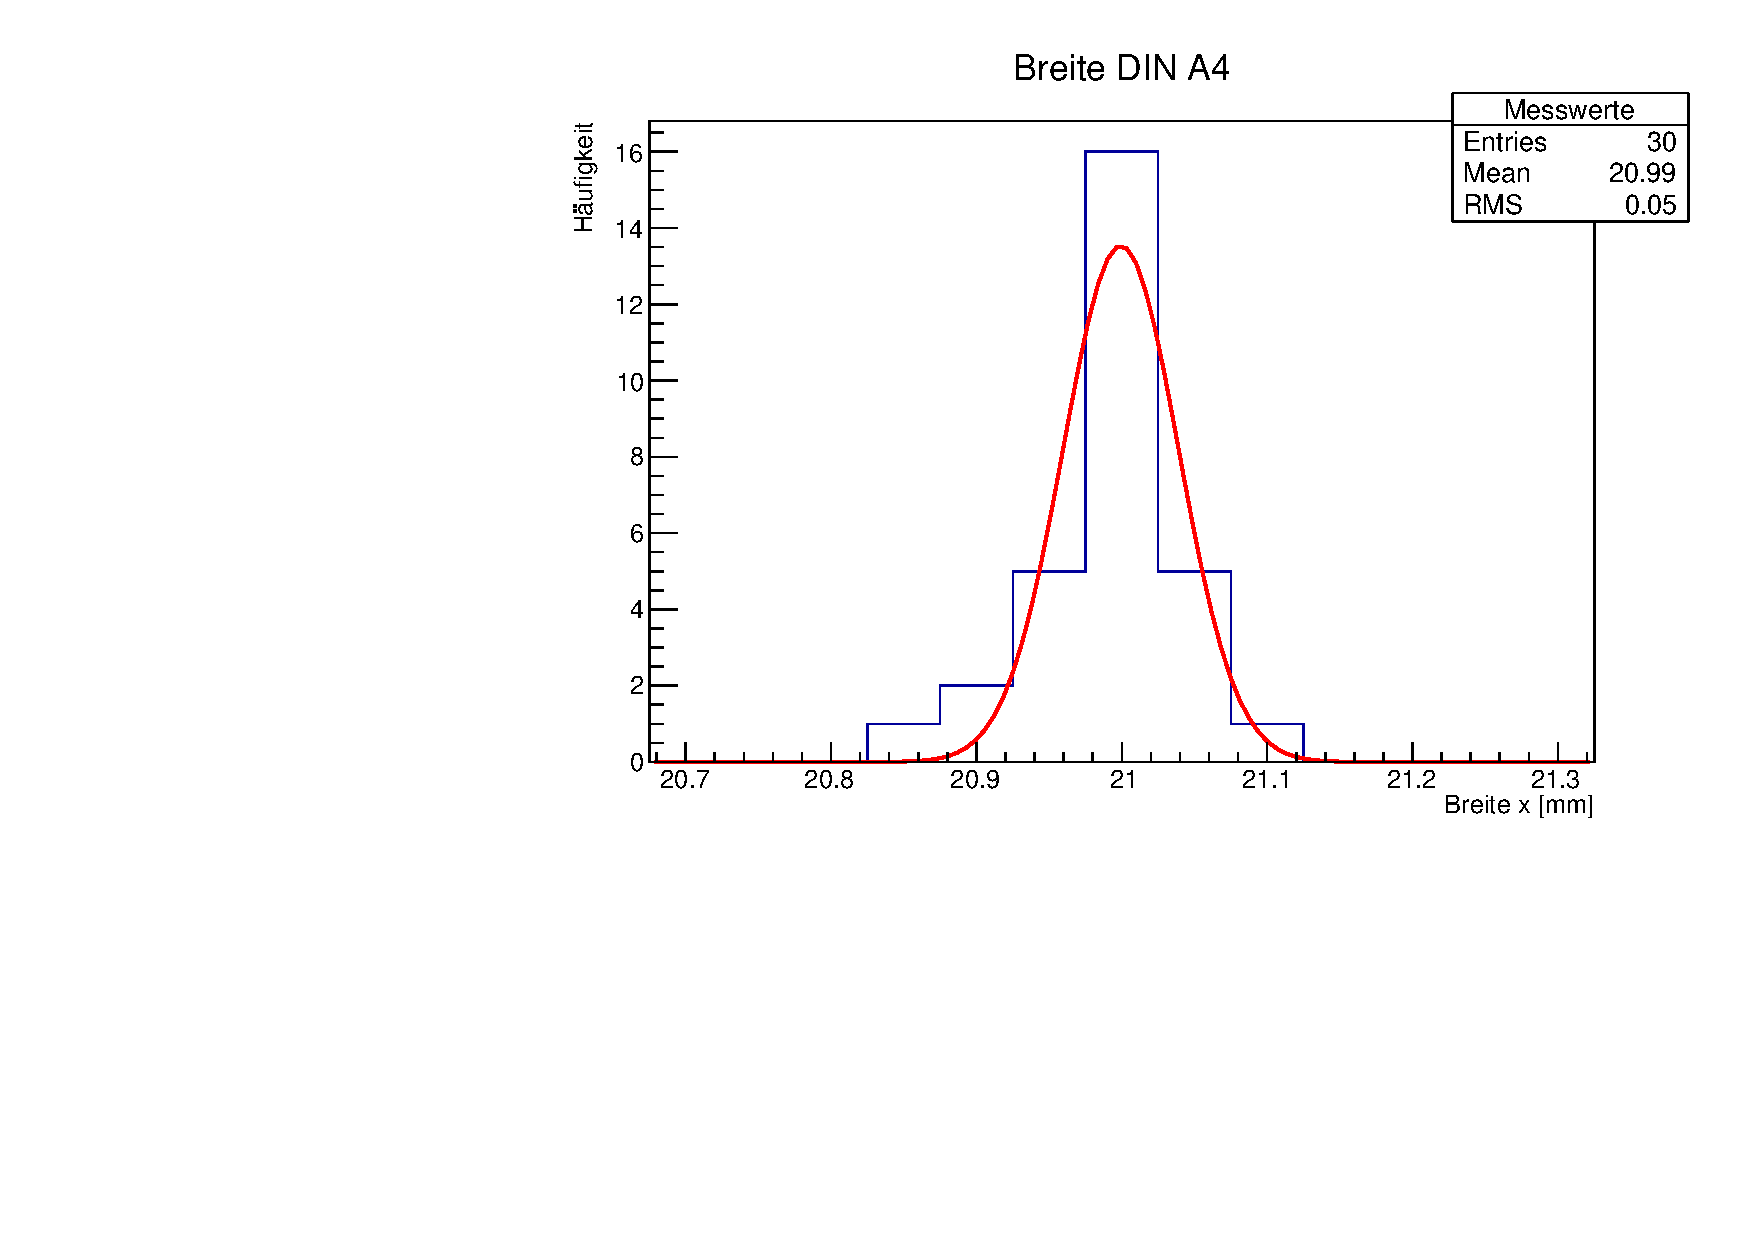
\includegraphics[width=1.00\textwidth]{00_einl/messung_histo.pdf}
	\captionof{figure}{Häufigkeitsverteilung der Messwerte aus Tabelle \ref{tab:MessungDINA4}}
	\label{fig:messung_histo}
\end{minipage}

Die Breite der Häufigkeitsverteilung wird durch die Standardabweichung $\sigma$ beschrieben, je größer diese ist, desto breiter ist die Kurve. Der Wendepunkt der Kurve befindet sich im Abstand $\sigma$ vom Mittelwert. Berechnet man die Fläche unter der Kurve zwischen den beiden Wendepunkten, so ergibt sich:
\begin{equation}
	\frac{1}{\sqrt{2\pi}\sigma}\int_{\bar{x}-\sigma}^{\bar{x}+\sigma}{e^{-\frac{\left(x-\bar{x}\right)^2}{2\sigma^2}}dx} = 0,683
\end{equation}

Das bedeutet, dass die Wahrscheinlichkeit, einen Messwert im Intervall $\left[\bar{x}-\sigma; \bar{x}+\sigma\right]$ zu finden (für $n\rightarrow\infty$), 68,3\% beträgt.

\noindent
Andere oft genutzte Intervalle sind:
\begin{align*}
	\mathrm{1-fache Standardabweichung} &\quad \phantom{0}\bar{x}-\sigma \; \mathrm{bis}\; \bar{x}+\sigma & (68,3\%)\\
	\mathrm{2-fache Standardabweichung} &\quad \bar{x}-2\sigma\; \mathrm{bis}\; \bar{x}+2\sigma & (95,5\%)\\
	\mathrm{3-fache Standardabweichung} &\quad \bar{x}-3\sigma\; \mathrm{bis}\; \bar{x}+3\sigma & (99,7\%)
\end{align*}
%**********************************************************************************************************************
\subsection{Die Unsicherheit eines Messergebnisses}

Da wir als Messergebnis den Mittelwert angeben, ist die Messunsicherheit definiert durch die Frage: \textit{Wie weit weicht der Mittelwert $\bar{x}$ aller Messungen vom wahren Wert $\mu$ ab?}

Diese Abweichung nimmt mit zunehmender Anzahl an Messungen immer weiter ab, der Mittelwert nähert sich dem wahren Wert immer mehr an. Bei einer großen Anzahl an Messungen gilt für die \textit{statistische Unsicherheit des Mittelwertes}:
\begin{important}
	\begin{equation}
		\Delta{\bar{x}} = \frac{\sigma_x}{\sqrt{n}}
	\end{equation}
\end{important}

Den Intervall $\left[\bar{x}-\Delta\bar{x}; \bar{x}+\Delta\bar{x}\right]$ nennt man den \textit{Konfidenzbereich auf dem Vertrauensniveau 68,3\%}. Die Aussage ''Der Messwert beträgt $\bar{x}\pm\Delta\bar{x}$'' bedeutet, dass wenn man den Messvorgang wiederholen würde (mit der gleichen Anzahl an Einzelmessungen $n$), für mindestens $68,3\%$ der auf Grundlage der Messdaten berechneten Konfidenzintervalle der wahre Wert im jeweiligen Konfidenzintervall liegt.

\paragraph{Bemerkung:} Korrektur für kleine Anzahl von Messungen

\begin{table}[t]	
	\centering
		\begin{tabular}[t]{|c|c|c|c|} 
			 & 68,3\% & 95\% & 99,7\% \\ 
			n & t & t & t \\\hline
			2 & 1,84 & 12,71 & 235,8 \\
			3 & 1,32 & 4,30 & 19,21 \\
			4 & 1,20 & 3,18 & 9,22 \\
			5 & 1,15 & 2,78 & 6,62 \\
			6 & 1,11 & 2,57 & 5,51 \\
			8 & 1,08 & 2,37 & 4,53 \\
			10 & 1,06 & 2,26 & 4,09 \\
			20 & 1,03 & 2,09 & 3,45 \\
			30 & 1,02 & 2,05 & 3,28 \\
			50 & 1,01 & 2,01 & 3,16 \\
			100 & 1,00 & 1,98 & 3,08 \\
			200 & 1,00 & 1,97 & 3,04 
		\end{tabular}
	\captionof{table}{Werte der Student-t-Verteilung für verschiedene Konfidenzintervalle}
	\label{tab:Student-t}
\end{table}

\noindent
Liegen nur wenige Messungen vor, so ist die Annahme nicht mehr wahr, dass die Verteilung der Messwerte durch die Normalverteilung beschrieben wird. Stattdessen muss die Student-t-Verteilung verwendet werden. Den Unterschied der beiden Verteilungen berücksichtigen wir durch einen Korrekturfaktor $t$, der Tabelle \ref{tab:Student-t} entnommen werden kann.

\noindent
Für die Unsicherheit des Messwertes gilt dann:
\begin{equation}
 \Delta \bar{x} = \frac{t}{\sqrt{n}}\sigma_x = t\cdot \sigma_{\bar{x}}
\end{equation}

Wie man sieht, geht der Korrekturfaktor für $n\rightarrow\infty$ gegen $t=1$, denn für große Anzahlen an Einzelmessungen nähert sich die Student-t-Verteilung der Normalverteilung an.

%**********************************************************************************************************************
\subsection{Der gewichtete Mittelwert und seine Unsicherheit}

Bei der Bildung des arithmetischen Mittelwertes geht man implizit davon aus, dass alle Messwerte, die in die Mittelung aufgenommen werden, dieselbe Unsicherheit haben. Dies muss nicht immer der Fall sein.\\

Beispiel: \textit{Aus irgendeinem Grund verwenden Sie zur Messung derselben Länge unterschiedliche Maßstäbe. Z. Bsp. benutzen Sie für einige Messungen ein Lineal mit einer Genauigkeit von 1~mm, für andere Messungen eine Schieblehre, die eine Auflösung von 0,1~mm hat.}\\

Um diese unterschiedlich genauen Messungen sinnvoll in einem Mittelwert zu kombinieren, benutzt man den \textit{gewichteten Mittelwert}:
\begin{important}
	\begin{equation}
		\bar{x} = \frac{\sum_{i=1}^n{w_i\cdot x_i}}{\sum_{i=1}^n{w_i}}
	\end{equation}
\end{important}
wobei die Wichtungsfaktoren $w_i$ die Kehrwerte der Abweichungsquadrate sind:
\begin{equation*}
	w_i = \frac{1}{\Delta x_i^2}
\end{equation*}
Auf diese Weise tragen Messwerte mit größerer Unsicherheit weniger stark zum Mittelwert bei. Die Unsicherheit des gewichteten Mittelwertes beträgt:
\begin{equation}
	\Delta\bar{x} = \frac{1}{\sum_{i=1}^n{w_i}}
\end{equation}
Sind alle Wichtungsfaktoren $w_i$ gleich, geht der gewichtete Mittelwert in den 'normalen` über, und dessen Abweichung sinkt wieder mit der Wurzel der Zahl der Werte.\\

Der gewichtete Mittelwert gilt strenggenommen nur für normalverteilte Größen. Er wird aber mangels Alternativen auch auf andere statistische oder systematische Abweichungen angewandt. Vor einer Anwendung ist aber zu prüfen, ob die unterschiedlichen Messungen mit dem zugehörigen Konfidenzbereich überlappen. Falls dies nicht der Fall ist, liegt eine zusätzliche, nicht erkannte Abweichung vor (z.B. grobe Fehler).\\

Beispiel:
\textit{Drei Praktikumsgruppen erhalten die Aufgabe, den Durchmesser einer Dose zu bestimmen. Die erste Gruppe erhält eine Schieblehre als Hilfsmittel, die zweite ein 30~cm langes Lineal mit Millimeterskala und die Studierenden der dritten Gruppe müssen mit bloßem Auge den Durchmesser abschätzen:}

\begin{tabular}{|l|l|l|l|} \hline
		& Gruppe 1: & Gruppe 2: & Gruppe 3:\\
		& Durchmesser [mm] & Durchmesser [mm] & Durchmesser [cm]\\ \hline
	Messung 1 & 100,3 & 102,5 & 8 \\
	Messung 2 & 100,2 & 105,0 & 9\\
	Messung 3 & 100,4 & 102,0 & 10 \\
	Messung 4 & 100,1 & 107,0 & 13 \\
	Messung 5 & 100,2 & 100,5 & 6 \\
	Messung 6 & 100,3 & 101,0 & 12 \\
	Messung 7 & 100,5 & 102,5 & 9\\
	Messung 8 & 100,0 & 103,0 & 11\\
	Messung 9 & 100,4 & 102,5 & 12\\
	Messung 10 & 100,3 & 103,5 & 8 \\ \hline
	Mittelwert & 100,270 & 102,95 & 9,8\\ \hline
	Std. abw. & 0,047 & 0,60 & 0,70\\ \hline
\end{tabular}

\textit{Der Mittelwert aus allen diesen Messungen für den Dosendurchmesser $d$ ergibt:}
\begin{align}
	\bar{d} & = \frac{\frac{100,27}{0,047^2}+\frac{102,95}{0,60^2}+\frac{98}{7^2}}{\frac{1}{0,047^2}+\frac{1}{0,60^2}+\frac{1}{7^2}}\;\mathrm{mm} = 100,286\;\mathrm{mm}\\
	\Delta\bar{d} & = \frac{1}{\sqrt{\frac{1}{0,047^2}+\frac{1}{0,60^2}+\frac{1}{7^2}}}\;\mathrm{mm} = 0,047\;\mathrm{mm}
\end{align}
\textit{Als Messwert für den Durchmesser ergibt sich also: $d = (100,286\pm 0,047)\;\mathrm{mm}$.}
%**************************************************************
% Hier noch was zu Geräten und Aufspüren systematischer Fehler?
%**************************************************************

%**********************************************************************************************************************
%**********************************************************************************************************************
\section{Indirekte Messung: Fehlerfortpflanzung}

Wenn sich die gesuchte Größe aus zwei oder mehr einzeln gemessenen Größen zusammensetzt, so nennt man die Bestimmung der zusammengesetzten Größe eine \textit{indirekte Messung}. Ein Beispiel dafür ist schon die einfache Bestimmung der Fläche eines DIN A4 Blattes, die wir uns früher schon angeschaut haben.

Wie wir wissen, sind die einzelnen, direkten Messungen mit Unsicherheiten behaftet. Wie können wir aus diesen die Ungenauigkeit der indirekten Messung der zusammengesetzten Größe berechnen?

%**********************************************************************************************************************
\subsection{Größtfehlerbetrachtung}

Die einfachste Möglichkeit, den Fehler abzuschätzen, ist die Annahme, dass die Unsicherheiten aller Einzelgrößen voll zur Gesamtunsicherheit beitragen und sich nicht untereinander beeinflussen (man sagt \textit{sie sind nicht korreliert}).

Rechnerisch wird das umgesetzt, indem man in die Formel zur Berechnung der gesuchten zusammengesetzten Größe die Einzelmessungen $x_i \pm \Delta x_i$ so einsetzt, dass das Ergebnis maximal wird. Anschließend wird der Vorgang so wiederholt, dass das Ergebnis minimal wird. Die Differenz der beiden Ergebnisse bezeichnet man als den \textit{Größtfehler}.\\

%\noindent
Dieses Verfahren berücksichtigt den statistischen Zusammenhang der einzelnen Beiträge nicht, daher liefert es im Allgemeinen zu große Werte für die Unsicherheit. Darüber hinaus können sich rechnerische Schwierigkeiten ergeben, wenn z. Bsp. die entsprechende Größe in einer Summe im Nenner und im Zähler der Formel vorkommt. In diesem Fall ist es schwierig herauszufinden, ob die positive oder die negative Abweichung den größten bzw. den kleinsten Wert ergibt. Dieses Verfahren ist daher nur für den Notfall geeignet, liefert jedoch oft eine brauchbare Abschätzung.

%**********************************************************************************************************************
\subsection{Gauß'sche Fehlerfortpflanzung}

Betrachten wir eine Größe $g$, die nicht direkt gemessen werden kann, sich aber aus mehreren direkt gemessenen Größen $x$, $y$, $z$,... berechnen läßt:
\begin{equation}
	g = g(x,y,z,...)
\end{equation}
Der Einfachheit halber wollen wir uns im Folgenden auf die drei Messgrößen $x$, $y$ und $z$ beschränken, die Rechnungen können jedoch prinzipiell mit beliebig vielen Messgrößen durchgeführt werden.

Wir gehen davon aus, dass die Messserien für die Größen $x$, $y$ und $z$ normalverteilt sind. Dann kann der Mittelwert $\bar{g}$ der gesuchten Größe bestimmt werden, indem man die Mittelwerte der Messgrößen in die Formel einsetzt:
\begin{important}
	\begin{equation}
		\bar{g} = g(\bar{x},\bar{y},\bar{z})
	\end{equation}
\end{important}

Wenn die Messgrößen $x$, $y$ und $z$ statistisch unabhängig voneinander sind, man sagt \textit{unkorreliert}, dann kann die gesamte Unsicherheit wie folgt berechnet werden:
\begin{important}
	\begin{equation}
		\Delta\bar{g} = \sqrt{\Delta\bar{x}^2 \cdot \left(\frac{\partial g}{\partial x} \right)^2_{\bar{x},\bar{y},\bar{z}} + \Delta\bar{y}^2 \cdot \left(\frac{\partial g}{\partial y} \right)^2_{\bar{x},\bar{y},\bar{z}} + \Delta\bar{z}^2 \cdot \left(\frac{\partial g}{\partial z} \right)^2_{\bar{x},\bar{y},\bar{z}}}
	\end{equation}
\end{important}

Diese Formel ist bekannt als die \textit{Gauß'sche Fehlerfortpflanzung}, wenn für die Unsicherheiten $\Delta\bar{x}$, $\Delta\bar{y}$, $\Delta\bar{z}$ die jeweilige Standardabweichung eingesetzt wird.

Die Ausdrücke $\partial g/\partial x$, $\partial g/\partial y$ und $\partial g/\partial z$ stehen dabei für die partiellen Ableitungen der Formel zur Berechnung von $g$ nach den Variablen $x$, $y$ und $z$.

\paragraph{Beispiel:} Messung der Dichte eines Quaders\\
\textit{
Die Dichte eines Quaders ergibt sich aus seiner Masse $m$ und seinem Volumen $V = x\cdot y\cdot z$, wenn $x$, $y$ und $z$ die Kantenlängen sind, nach der Formel
\begin{equation}
	\rho = \frac{m}{V} = \frac{m}{x\cdot y\cdot z}
	\label{eq:Dichte}
\end{equation}
Bei der Messung der Masse und der Kantenlängen findet man die Werte $\bar{m}\pm \sigma_m$, $\bar{x}\pm \sigma_x$, $\bar{y}\pm \sigma_y$ und $\bar{z}\pm \sigma_z$. Die partielle Ableitung von Gleichung \ref{eq:Dichte} nach der Masse $m$ ist:
\begin{equation*}
	\frac{\partial \rho}{\partial m} = \frac{1}{x\cdot y\cdot z}
\end{equation*}
Die partielle Ableitung nach $x$ lautet (für die anderen beiden Richtungen genauso vorgehen):
\begin{equation*}
	\frac{\partial \rho}{\partial x} = -\frac{1}{x}\cdot\frac{m}{x\cdot y\cdot z}
\end{equation*}
Damit ergibt sich für die Unsicherheit der Dichte:
\begin{equation}
	\Delta\bar{\rho} = \sqrt{\Delta\bar{x}^2\left(-\frac{1}{\bar{x}}\frac{m}{\bar{x}\bar{y}\bar{z}} \right)^2 + \Delta\bar{y}^2\left(-\frac{1}{\bar{y}}\frac{m}{\bar{x}\bar{y}\bar{z}} \right)^2 + \Delta\bar{z}^2\left(-\frac{1}{\bar{z}}\frac{m}{\bar{x}\bar{y}\bar{z}} \right)^2 + \Delta\bar{m}^2\left(\frac{1}{\bar{x}\bar{y}\bar{z}}\right)^2}
\end{equation}
In diese Gleichung sind jetzt nur noch die jeweiligen Mittelwerte und Unsicherheiten einzusetzen, um die Unsicherheit der Dichte zu berechnen.
}\\

Falls die einzelnen Messgrößen nicht normalverteilt sind, oder wenn sie nicht statistisch von einander unabhängig sind, muss man bei der Fortpflanzung der Unsicherheiten noch einen Korrekturfaktor berücksichtigen, der diese Korrelation der Messgrößen beschreibt. Diesen nennt man den \textit{Korrelationskoeffizienten}.

%**********************************************************************************************************************
\subsection{Fortpflanzung systematischer Abweichungen}

Systematische Abweichungen entziehen sich naturgemäß einer statistischen Behandlung. Man kann insbesondere nicht davon ausgehen, dass es unwahrscheinlich ist,
dass alle Abweichungen der Beteiligten Einzelgrößen gleichzeitig extremal sind.\\

Beispiel:
\textit{Eine Veränderung der Umgebungstemperatur bei der Messung zieht eine Abweichung aller Längenmessungen gemeinsam nach sich, da der Maßstab natürlich bei jeder Messung
'falsch' ist. Man muss also in diesem Fall davon ausgehen, dass die Abweichungen nicht quadratisch addiert werden dürfen, sondern linear addiert werden müssen. Der Einfluss jeder
Einzelabweichung muss voll auf die Gesamtabweichung durchschlagen.}\\

\textit{Im Fall einer systematischen Abweichung der Längenmessung durch einen nicht gleichmäßig geteilten Maßstab erscheint es jedoch sinnvoll anzunehmen, dass je nach Position die Abweichung unterschiedlich ist. Entsprechend kann man auch davon ausgehen, dass nicht gerade alle Abweichungen zum gleichen Zeitpunkt in die gleiche Richtung gehen. Hier ist also eine quadratische Addition sinnvoll.}\\

Es hängt also vom Einzelfall ab welche Methode der Fortpflanzung bei einer systematischen Abweichung angewandt werden muss. Die lineare Addition bei potentiell statistisch gekoppelten Vorgängen oder die quadratische Addition bei definitiv statistisch unabhängigen Vorgängen.\\
Sei beispielsweise die Größe $g$ aus drei Variablen $x, y, z$ zusammengesetzt, die jeweils die systematischen Unsicherheiten $\Delta x, \Delta y, \Delta z$ haben. Dann erfolgen lineare und quadratische Addition wie folgt:

\textbf{Lineare Addition}
\begin{equation} \label{eq:error_lin_add}
	\Delta\bar{g} = \left|\Delta\bar{x}\cdot \left[\frac{\partial g}{\partial x}\right]_{\bar{x}, \bar{y}, \bar{z}}\right|
								+ \left|\Delta\bar{y}\cdot \left[\frac{\partial g}{\partial y}\right]_{\bar{x}, \bar{y}, \bar{z}}\right|
								+ \left|\Delta\bar{z}\cdot \left[\frac{\partial g}{\partial z}\right]_{\bar{x}, \bar{y}, \bar{z}}\right|
\end{equation}

\textbf{Quadratische Addition}
\begin{equation} \label{eq:error_quad_add}
	\Delta\bar{g} = \sqrt{\Delta\bar{x}^2\cdot \left[\frac{\partial g}{\partial x}\right]^2_{\bar{x}, \bar{y}, \bar{z}}
											+ \Delta\bar{y}^2\cdot \left[\frac{\partial g}{\partial y}\right]^2_{\bar{x}, \bar{y}, \bar{z}}
											+ \Delta\bar{z}^2\cdot \left[\frac{\partial g}{\partial z}\right]^2_{\bar{x}, \bar{y}, \bar{z}}}
\end{equation}
%**********************************************************************************************************************
\subsection{Verknüpfung statistischer und systematischer Unsicherheiten}

Auch bei der Verknüpfung systematischer und statistischer Unsicherheiten ist die Frage nach de Kopplung der Gr"o{\ss}en zu beachten. Die Frage, ob die statistische Unsicherheit von der systematischen Abweichung abhängig ist oder nicht, ist jedoch letztlich nicht beantwortbar. Entsprechend werden in der Literatur auch beide Meinungen vertreten.\\

\noindent
\textbf{Im Praktikum} wollen wir vom konservativen Fall ausgehen und annehmen, dass die beiden Beitr"age nicht voneinander unabh"angig sind und befolgen die folgenden Schritte:
\begin{enumerate}
	\item Bestimmung der statistischen Unsicherheit aus allen Einzelgrößen mittels \textit{quadratischer Addition} nach Gleichung \ref{eq:error_quad_add}.
	\item Bestimmung der systematischen Unsicherheit aus \textit{linearer Addition} aller Einzelgrößen nach Gleichung \ref{eq:error_lin_add}.
	\item Verknüpfung der statistischen und systematischen Unsicherheit mittels normaler linearer Addition, nicht Gleichung \ref{eq:error_lin_add}, zur Gesamtunsicherheit, welche dann beim Ergebnis angegeben wird.
\end{enumerate}
%**********************************************************************************************************************
%\begin{todo}
	%Einen Abschnitt über systematische Unsicherheiten und wie man sie abschätzt.
%\end{todo}

%**********************************************************************************************************************
%**********************************************************************************************************************
%\section{Graphische Auswertung bei korrelierten Messwerten}
%
%Dein einfachste Beziehung zwischen zwei Messgrößen ist die \textit{lineare Abhängigkeit}
%\begin{equation}
	%y(x) = a\cdot x + b
%\end{equation}
%mit den beiden freien Parametern $a$ und $b$.
\chapter{Fehlerrechnung und Auswertungen im Praktikum} \label{v:fehler}

\section{Allgemeines}

Dieser Abschnitt m"usste eigentlich richtiger hei"sen: "`Rechnen mit
Ungenauigkeiten"'\index{Ungenauigkeiten}. Im Folgenden sollen kurz
einige Grundlagen zur Fehlerrechnung\index{Fehlerrechnung},
Statistik\index{Statistik} und Auswertung von
Messdaten\index{Auswertung} dargelegt werden, soweit sie f"ur
dieses Praktikum wichtig sind. F"ur eine genauere Betrachtung sei
auf die Spezialliteratur
%\cite{beving,bron,npp,kamke,physmess,lichten,tbstat,tbnum,taylor,messunsicher}
verwiesen.\\

\noindent
Dieser Abschnitt ist der Praktikumsanleitung für Physiker entnommen. Inhaltlich sollte er größtenteils mit dem vorherigen Abschnitt übereinstimmen, führt aber einige der Konzepte in größerer Tiefe ein.

\section{Vorbemerkung}

Eine physikalische Gr"o"se\index{Gr"o"se!Physikalische} kennzeichnet
Eigenschaften und beschreibt Zust"ande sowie Zustands"anderungen von
Objekten der Umwelt. Sie muss nach einer Forderung von
\person{Einstein} messbar sein. Die Vereinbarung, nach der die
beobachtete physikalische Einheit quantifiziert wird, ist die
Einheit der physikalischen Gr"o"se. Somit besteht eine physikalische
Gr"o"se {\bf G} immer aus einer quantitativen Aussage G (Zahlenwert)
und einer qualitativen Aussage [G] (Einheit): {\bf G} = G $\cdot$
[G].

F"ur physikalische Gr"o"sen gilt: "`Physikalische Gr"o"se = Zahlenwert
$\cdot$ Einheit"', also bitte immer Einheiten angeben.\footnote{Die
Betreuerinnen sollen Protokolle mit fehlenden Einheiten
zur"uckgeben.} Gesetzlich vorgeschrieben ist die Verwendung des
\emph{Internationalen Einheitensystems
(SI-Einheiten)}\index{SI-Einheiten}. Im amtlichen und gesch"aftlichen
Verkehr d"urfen nur noch SI-Einheiten\index{Einheit} benutzt werden. Teilweise muss man als Naturwissenschaftler aber
auch mit anderen, "alteren Einheiten umgehen k"onnen (Bsp.: Torr,
Gau"s). %Einen sehr sch"onen "Ubersichtsartikel "uber physikalische
%Gr"o"sen, deren Nomenklatur und Einheiten, finden Sie in Ref.~\cite{codata}.

Die Messung einer physikalischen Gr"o"se\index{Gr"o"se!physikalische}
erfolgt %durch Vergleich der Einheit dieser Gr"o"se nach der
Messmethode der (SI-)Vereinbarung oder einem darauf aufbauenden
Messverfahren. Je nach Genauigkeit des Messverfahrens tritt ein
unterschiedlich grosser Messfehler (Ungenauigkeit, Abweichung) auf.
Dabei ist zwischen den \emph{systematischen}, f"ur das Messverfahren
charakteristischen Messfehlern\index{Messfehler} und den
\emph{zuf"alligen} oder \emph{statistischen}, vom einzelnen
Experiment abh"angigen Fehlern zu unterscheiden. Zu systematischen
Messfehlern geh"oren z.B. eine falsche Kalibrierung eines
Messger"ates, Ablesefehler (Parallaxe), falsche Justierung,
Messwertdrift, etc. Zu statistischen Fehlern geh"oren (zuf"allige)
Schwankungen wie elektronische Triggerschwankungen,
Temperaturschwankunken, Rauschen, ungenaues Anlegen von Ma"sst"aben
etc. Zur grafischen Analyse der Messwertschwankungen dient das
Histogramm. Bei zuf"alligen Messfehlern ist die H"aufigkeitsverteilung
der Messwerte $N_j(x_j)$ symmetrisch zu einem Mittelwert, dem
Erwartungswert $\mu$. Wird die Anzahl $n$ der Wiederholungsmessungen
stark erh"oht, so geht die (diskrete) relative H"aufigkeitsverteilung
$N_j(x_j) \rightarrow h(x)$ in eine glockenf"ormige Normalverteilung
(\person{Gau"s}sche Verteilungsfunktion) mit der
Halbwertsbreite\index{Halbwertsbreite} $\Gamma$ (= halbe Breite der Kurve
in halber H"ohe des Maximums, engl.~\textsc{HWHM=Half Width at Half
Maximum}) der Messwerte "uber:
%
\begin{important}
\begin{equation}\label{e:gaussnormal}
    h(x) = \frac{1}{\sqrt{2 \pi}\sigma} e^{-\frac{(x-\mu)^2}{2 \sigma^2}}
    \qquad \mbox{mit} \qquad
    \sigma = \frac{\Gamma}{\sqrt{2 \, \ln 2}} \, .
\end{equation}
\end{important}

Der Parameter $\sigma$ ist ein Ma"s f"ur die Breite der
Verteilungsfunktion $h(x)$: 68,3~\% der Messwerte liegen im Bereich
$\mu - \sigma < x < \mu + \sigma $. Aus der H"aufigkeitsverteilung $h(x_j)$
einer endlichen Anzahl $N$ von Messungen der $m$ diskreten
Messwerte $x_1, \ldots x_m$ lassen sich f"ur 
$\mu$ und $\sigma$ nach der Theorie der
Beobachtungsfehler von \person{Gau"s} Sch"atzwerte berechnen.
Demnach ist die beste N"aherung f"ur $\mu$ der arithmetische
Mittelwert $\bar{x}$, f"ur $\sigma$ die
Standardabweichung $s$, die sich aus der
Fehlersumme berechnet (s.u.). 
%Letztere ist minimal, wenn der
%arithmetische Mittelwert als Erwartungswert gesetzt wird (siehe
%unten).

\section{Ungenauigkeiten und Fehler}

Alle Messvorg"ange liefern Messergebnisse mit einem Fehler, der
nach einer verbindlichen "Ubereinkunft ein Ma"s f"ur die Genauigkeit
des Messergebnisses darstellt. Ein Beispiel: Die L"ange eines
Stabes wird durch Anlegen eines Ma"sstabes bestimmt. Dann sind zwei
Arten von Fehlern m"oglich:
%
\begin{enumerate}
  \item der systematische Fehler des Ma"sstabs, der sich durch genauen Vergleich
   mit dem Urmeter\index{Urmeter} ermitteln l"asst,
  \item der zuf"allige Fehler, der sich durch Unsicherheiten beim Anlegen des
 Ma"sstabs ergibt.
\end{enumerate}

Alle Messergebnisse m"ussen deshalb mit Fehlerangabe $\bar{x} \pm
\Delta x$ angeben werden. In den meisten
F"allen darf man annehmen, dass die Messwerte um den wahren Wert
statistisch streuen, d.h. dass die Abweichungen im Betrag
schwanken und im Mittel gleich oft positiv wie negativ
ausschlagen. Dann ist der beste Wert (Bestwert)\index{Bestwert},
den man aufgrund von $n$ wiederholten Messungen mit Messergebnis
$x_i$ angeben kann, der Mittelwert\index{Mittelwert} $\bar{x}$:
%
\begin{important}
\begin{equation}\label{e:mw}
\mbox{Mittelwert: } \,  \bar{x} = \frac{1}{n} \sum_{i=1}^n x_i \,
.
\end{equation}
\end{important}
%
Au"ser den Streufehlern, die man auch zuf"allige - oder statistische
- Fehler nennt, treten gew"ohnlich auch so genannte systematische
Fehler auf. Ist ein Messger"at falsch kalibriert, wird es zum
Beispiel immer zu gro"se Werte liefern. Um eine Aussage "uber die
Zuverl"assigkeit des Messergebnisses machen zu k"onnen, muss die
Gr"o"se dieser beiden Fehlereinfl"usse abgesch"atzt werden. Die
Aufgabe der Fehlerrechnung ist also die Bestimmung des Fehlers
$\Delta x = \Delta x_{\rm syst.} + \Delta x_{\rm stat.}$. Das Ergebnis der
Messung mit Fehlerangabe\index{Fehlerangabe} lautet dann:
%
\begin{equation}\label{e:ergfehler}
  \mbox{Ergebnis mit Fehlerangabe: } \,  \bar{x} \pm \Delta x \, .
\end{equation}
%
Diese Angabe bedeutet: Man erwartet, dass der wahre Wert $x_w$ im
Bereich $\bar{x} - \Delta x \leq x_w \leq \bar{x} + \Delta x $
liegt. $\Delta x$ nennt man den absoluten Fehler. Es kann auch der
relative Fehler angegeben werden: $\Delta x / \bar{x}$.

Da jede gemessene physikalische Gr"o"se mit einem Fehler behaftet ist,
macht es keinen Sinn als Ergebnis eine Zahl mit vielen Ziffern
anzugeben. Die Zahl der angegebenen Ziffern sollte an die Gr"o"se des
Fehlers angeglichen werden, d.h. das Ergebnis ist entsprechend
sinnvoll zu runden. Das Ergebnis und der Fehler werden an der
gleichen Stelle gerundet. Der Fehler wird normal gerundet.


\section{Systematische Fehler}

Systematische Fehler\index{Fehler!systematische} bei Messungen im
Praktikum r"uhren haupts"achlich von Ungenauigkeiten der Messger"ate
oder der Messverfahren her. Abweichungen der Messbedingungen, wie
z.B. der Temperatur, spielen in der Regel eine untergeordnete
Rolle. Beispiele f"ur systematische Fehler sind:
%
\begin{itemize}
  \item Eine Stoppuhr geht stets vor oder nach
  \item Ein Voltmeter zeigt wegen eines Kalibrierfehlers einen stets zu gro"sen
   (oder zu kleinen) Wert an
  \item Der Ohmsche Widerstand in einer Schaltung weicht vom
  angegebenen Nominalwert ab.
  \item Eine Beeinflussung der Messung durch Messger"ate (z.B.
  Innenwiderst"ande) wird nicht ber"ucksichtigt.
\end{itemize}
%
Systematische Fehler haben stets einen festen Betrag und ein
eindeutiges Vorzeichen. Sie "andern sich auch nicht, wenn die Messung
mit der gleichen Anordnung und den gleichen Ger"aten wiederholt wird.
Da das Vorzeichen nicht bekannt ist, muss man sie auch mit dem
unbestimmten Vorzeichen $\pm$ angeben. F"ur die Absch"atzung des
Betrages gelten die folgenden Hinweise.

F"ur Messger"ate sind die maximal erlaubten Abweichungen $\Delta
x_{\rm syst.}$ einer Anzeige $x$ vom wahren Wert in der Regel durch
Herstellungsnormen festgelegt (G"ute des Ger"ates, siehe
Beschreibung bei "`Messger"aten"'). F"ur elektrische Messger"ate ist
der Begriff "`G"uteklasse"' eingef"uhrt worden. Diese gibt den
erlaubten systematischen Fehler als Prozentwert vom Vollausschlag
an. Diesen Fehler setzt man dann f"ur alle Messungen in diesem
Messbereich an.

Bei L"angenmessger"aten betr"agt der m"ogliche systematische Fehler
selten mehr als wenige Promille vom Messwert und kann daher
gegen"uber den Streufehlern in den meisten F"allen vernachl"assigt
werden. F"ur eine quantitative Absch"atzung kann die folgende Formel
verwendet werden:
%
\begin{equation}\label{e:skalafehler}
  \frac{\Delta x_{\rm syst}}{x} =
  \frac{\mbox{1 Skalenteil der Skala}}{\mbox{Skalenteile bei Vollausschlag.}}
\end{equation}

Stoppuhren sind noch genauer und Ihr Fehler kann zu $\Delta
x_{\rm syst} = \mbox{kleinster Skalenwert} + {\rm 0.005} \cdot
\mbox{Messwert} $ abgesch"atzt werden.

Bei der Messung von Temperaturen mit einem Fl"ussigkeitsthermometer
betr"agt der Ger"atefehler etwa 1~Strichabstand.


\section{Statistische, zuf"allige Fehler}

Ursachen f"ur zuf"allige Fehler\index{Fehler!statistische} sind z.B.
Schwankungen der Messbedingungen w"ahrend der Messung oder auch
Ungenauigkeiten bei der Ablesung von Messinstrumenten (z.B.
Parallaxe). Um den Betrag des Streufehlers absch"atzen zu k"onnen,
wiederholt man die Messung mehrfach. Ein Ma"s f"ur die Streuung kann
dann aus den Abweichungen $x_i - \bar{x}$ der einzelnen Messwerte
vom Mittelwert gewonnen werden, die von Gau"s als
Standardabweichung $s$ f"ur $n$ Messungen $x_i$ definiert wurde:
%
\begin{equation}\label{e:standabw}
  s = \sqrt{ \frac{1}{n-1} \sum_{i=1}^n \left( x_i - \bar{x} \right)^2 }
\end{equation}

Die Standardabweichung $s$ repr"asentiert die Genauigkeit der
einzelnen Messung und damit auch des Messverfahrens. Deshalb wird
$s$ auch als mittlerer quadratischer Fehler der Einzelmessung
bezeichnet. Je mehr Einzelmessungen vorliegen, umso genauer wird
der Mittelwert sein. Der mittlere quadratische Fehler des
Mittelwertes $\Delta x_{\rm stat.}$ ist nach der Fehlertheorie um den
Faktor $\nicefrac{1}{\sqrt{n}}$ kleiner.
%
\begin{important}
\begin{equation}\label{e:fmw}
 \Delta x_{\rm stat} = \frac{s}{\sqrt{n}}
     = \sqrt{ \frac{1}{n(n-1)} \sum_{i=1}^n \left( x_i - \bar{x} \right)^2 }
\end{equation}
\end{important}
%
Dieser Wert $\Delta x_{\rm stat}$ wird manchmal in Anlehnung an
die Normalverteilung als $\sigma_{\bar{x}}$ bezeichnet. 
Dabei sollte der Wert $\sigma_{\bar{x}}$, der den Fehler auf
den arithmetischen Mittelwert $\bar{x}$ angibt, {\it nicht} mit dem
Fehler $\sigma=s$ der Einzelmessung $x_i$ verwechselt werden!
Die Fehlerrechnung
erlaubt dann die Aussage (wenn systematische Fehler wesentlich
kleiner sind), dass der wahre Wert mit einer Wahrscheinlichkeit
von 68\% im Intervall mit der Breite $\sigma_{\bar{x}}$ um den Mittelwert
liegt: $\bar{x} - \sigma_{\bar{x}} < x_w < \bar{x} + \sigma_{\bar{x}} $.

%Nach der Theorie der Beobachtungsfehler (t-Verteilung nach
%Student, alias \person{W. S. Gosset}) sind bei normalverteilten
%Messgr"ossen die Vertrauensgrenzen abh"angig von der Anzahl $n$ der
%Messungen und der Standardabweichung $s$ des Messverfahrens:
%
%\begin{equation}\label{e:t-vert}
%    x = \bar{x} \pm t_P \cdot \frac{s}{\sqrt{n}}
%\end{equation}
%
%Der Faktor $t_P$ folgt aus der Student-t-Verteilung und ist
%abh"angig von der Anzahl der Wiederholungsmessungen und der
%geforderten statistischen Sicherheit $P$
%\cite{bron,tbstat}. F"ur gro"se $n$ entspricht
%$t_{\numprint[\%]{68.3}}$=1. %, d.h. $\Delta x = \Delta \bar{x}$.
%Einige Werte f"ur $t_P$ sind in Tabelle~\ref{t:student} aufgef"uhrt.

Im Praktikum, wie meistens in der
Physik, k"onnen wir uns mit 1$\sigma$, also 68,3~\% Sicherheit zufrieden geben.
Bitte geben Sie Ihre Ergebnisse in den Protokollen auch so an,
d.h. benutzen Sie die $1\sigma$"=Regel f"ur Ihre Fehlerangaben.
Liegt neben der statistischen Unsicherheit auch noch ein
systematischer Fehler vor, so ist als Gesamt-Messfehler die quadratische Summe
der beiden Fehler anzugeben.
%
%\begin{table}[htb]%
%  \centering%
%  \caption[Student-Verteilung: Werte von $t_P$]{\label{t:student}Einige Werte
%  von $t_P$ bei der Student"=t"=Verteilung
%   f"ur die angegebene statistische Sicherheit.}%
%  \begin{tabular}{rrrr}%
%    \toprule
%    $n$ & 68.3\% & 95\% & 99.7\% \\ \midrule
%    3   & 1.32 & 4.3 & 19.2 \\
%    5   & 1.15 & 2.8 & 6.6\\
%    10  & 1.06 & 2.3 & 4.1\\
%    100 & 1.00 & 2.0 & 3.1\\ \bottomrule
%  \end{tabular}
%\end{table}


\section{Gewichteter Mittelwert}

Bei Vorliegen mehrerer \emph{unabh"angiger} Ergebnisse ist es "ublich,
den gewichteten Mittelwert\index{Mittelwert!gewichtet} anzugeben:
%
\begin{important}
\begin{equation}\label{e:gewmittel1}
 \bar x = \frac{
   \sum\limits_i \frac{x_i}{\sigma_i^2 }
    }{
    \sum\limits_i \frac{1}{\sigma_i^2}
    }
    \quad \mbox{mit Fehler: } \quad
    \sigma  = \sqrt{\frac{1}{\sum\limits_i \frac{1}{\sigma_i^2}} } \, .
\end{equation}
\end{important}
%
Bei stark unterschiedlich genauen Werten greift man besser auf
folgende Berechnung des Fehlers zur"uck:
%
\begin{equation}\label{e:gewsigma2}
 \sigma  = \sqrt {\frac{{\sum {\frac{{\left( {x_i  - \bar x}
 \right)^2 }}{{\sigma _i^2 }}} }}{{\left( {n - 1} \right)\sum
 {\frac{1}{{\sigma _i^2 }}} }}} \, ,
\end{equation}
%
oder nimmt das Maximum des mit den beiden obigen Formeln
berechneten Fehlers.

\section{Lineare Regression}

Hat man die Messwerte $y_i(x_i)$ vorliegen und vermutet einen
linearen Zusammenhang $y=m\cdot x + b$, so kann man dies einfach
mit der linearen Regression\index{Lineare Regression} testen. 

\subsection{Einfache Regression}

Ohne Ber"ucksichtigung bzw.~Kenntnis der Fehler auf die Messwerte 
$y_i$ ergibt sich f"ur die Steigung aus der linearen Regression:
%
\begin{equation}
m = \frac{{n\sum {x_i y_i  - \sum {x_i \sum {y_i } } } }}{{n\sum
{x_i^2  - \left( {\sum {x_i } } \right)^2 } }}
\end{equation}
%
und der Achsenabschnitt ist
%
\begin{equation}
b = \frac{{\sum {x_i^2 \sum {y_i }  - \sum {x_i \sum {x_i y_i } }
} }}{{n\sum {x_i^2  - \left( {\sum {x_i } } \right)^2 } }}
\end{equation}
%
Die jeweiligen Fehler berechnen sich zu:
%
\begin{equation}
\sigma_m^2  = \frac{{n\sum {\left( {y_i  - b - mx_i } \right)^2 }
}}{{\left( {n - 2} \right)\left( {n\sum {x_i^2  - \left( {\sum
{x_i } } \right)^2 } } \right)}}
\end{equation}
%
\begin{equation}
\sigma_b^2  = \frac{{\sum {x_i^2  \cdot } \sum {\left( {y_i  - b -
mx_i } \right)^2 } }}{{\left( {n - 2} \right)\left( {n\sum {x_i^2
- \left( {\sum {x_i } } \right)^2 } } \right)}}
\end{equation}
%
und der Korrelationskoeffizient\index{Korrelationskoeffizient}
berechnet sich folgenderma"sen:
%
\begin{equation}
 r = \frac{
 {n\sum {x_i y_i  - \sum {x_i \sum {y_i } } } }
 }
 {
 {\sqrt{n\sum {x_i^2  - \left( {\sum {x_i } } \right)^2 }} \cdot
  \sqrt{n\sum {y_i^2  - \left( {\sum {y_i } } \right)^2 } } }
 }
\end{equation}
%
Mathematisch liefert der Korrelationskoeffizient ein Ma{\ss} daf"ur, ob die Annahme eines linearen Zusammenhangs zwischen den $x_i$ und $y_i$ sinnvoll ist. Je dichter der Betrag des Korrelationskoeffizienten bei Eins liegt, desto besser ist die Linearit"at.\\
Man sei aber vorsichtig, aus einem guten $r$ sofort auf einen
wirklich physikalischen linearen Zusammenhang zu schlie"sen.

\subsection{Regression mit Messfehlern} \label{v:LinRegErr}

Unter der Voraussetzung, dass nur die
$y_i$-Werte mit dem Fehler $\sigma_i$ fehlerbehaftet, w"ahrend die
$x_i$-Werte fehlerfrei sind, ergibt sich f"ur die lineare Regression:
\begin{align*}
\Delta&=\sum{\frac{1}{\sigma_i^2}}\sum{\frac{x_i^2}{\sigma_i^2}}-
\left(\sum{\frac{x_i}{\sigma_i^2}}\right)^2 & &
\\
%
m&=\frac{1}{\Delta}\left(\sum{\frac{1}{\sigma_i^2}}
\sum{\frac{x_iy_i}{\sigma_i^2}}-\sum{\frac{x_i}{\sigma_i^2}}\sum{\frac{y_i}{\sigma_i^2}}
\right)
&\sigma_m&=\sqrt{\frac{1}{\Delta}\sum{\frac{1}{\sigma_i^2}}} \\
%
b&=\frac{1}{\Delta}\left(\sum{\frac{x_i^2}{\sigma_i^2}}
\sum{\frac{y_i}{\sigma_i^2}}-\sum{\frac{x_i}{\sigma_i^2}}\sum{\frac{x_iy_i}{\sigma_i^2}}
\right) \hspace{11mm}
&\sigma_b&=\sqrt{\frac{1}{\Delta}\sum{\frac{x_i^2}{\sigma_i^2}}} \\
%
\chi^2&=\sum{\left[\frac{1}{\sigma_i}\left(y_i-mx_i-b\right)\right]^2} & &
\end{align*}


\section{Mathematische Behandlung}

\subsection{Grundlagen der Fehlerrechnung: Bestwert und Fehler}

Wir betrachten im Folgenden einen vorher berechneten Mittelwert
aus Messergebnissen f"ur eine physikalische Gr"o"se und bezeichnen
diesen mit $M$. F"ur diese Gr"o"se $M$ kennen wir den wahren Wert
$M_W$, der in einem wirklichen Experiment nat"urlich unbekannt ist,
aber als existent angenommen werden kann. Jeder Messwert $M_i$ der
Gr"o"se $M$ weicht vom wahren Wert um den absoluten Fehler $\Delta M_i$
ab:
%
\begin{equation} \label{b}
 \Delta M_i = M_i - M_W \, .
\end{equation}
%
Das Endergebnis einer $n$-mal wiederholten Bestimmung von $M$ soll
durch einen Bestwert $M_B$ beschrieben werden, der der Vorschrift
%
\begin{equation} \label{c}
\sum_{i=1}^{n}\, (M_{i} - M_{B})^{2} = f(M_{B}) = \mbox{Minimum}
\end{equation}
%
gen"ugt, die als \person{Gau"s}sche Methode der kleinsten
(Fehler-)Quadrate zur Bestimmung des Bestwertes\index{Bestwert}
bezeichnet wird. F"uhrt man die Bestimmung des Minimums nach der
Vorschrift
%
\begin{equation} \label{d}
 \frac{d}{d M_B} \sum_{i=1}^{n}(M_{i} - M_{B})^{2} = 0
\end{equation}
%
aus, so ergibt sich
%
\begin{equation} \label{e}
 M_{B} = \frac{1}{n} \sum_{i=1}^{n} M_{i} = \bar M
\end{equation}
%
und damit die Definition:
%
\begin{definition} \label{def:bestwert}
  Der Bestwert ist gleich dem arithmetischen Mittel.
\end{definition}

Der in (\ref{b}) definierte absolute Fehler der
Einzelmessung\index{Fehler!der Einzelmessung} l"asst sich in der
Praxis nicht ermitteln. Deshalb f"uhren wir nach der Vorschrift
%
\begin{equation} \label{f}
 \Delta M = \sqrt{
  \frac{1}{n-1} \sum_{i=1}^{n} \left( M_{i} - M_{B} \right)^{2}
 }
\end{equation}
%
den mittleren quadratischen Fehler der Einzelmessung ein. Der in
(\ref{f}) eigentlich erwartete Gewichtsfaktor $1/n$ wurde durch
$1/(n-1)$ ersetzt, weil man f"ur 1~Messwert nat"urlich keinen Fehler
berechnen kann.


\subsection{Die Normalverteilung}

Normalerweise sind die Messdaten $M_i$ gen"ahert in Form einer
Glockenkurve um den wahren Wert $M_W$, angen"ahert durch den
Bestwert $M_B$, verteilt. Die mathematische Form der
Glockenkurve\index{Glockenkurve} ist gegeben durch die
\person{Gau"s}sche
Normalverteilung\index{Normalverteilung}\index{Gau"s}:
%
\begin{important}
\begin{equation} \label{g}
  P(x) =
  \frac{1}{\sqrt{2\pi} \sigma} \cdot
  \exp\left( -\frac{(x-\bar{x})^{2}}{2\sigma^{2}} \right)
\end{equation}
\end{important}
%
wobei $x = M_i - M_B$ gesetzt wurde und somit hier $\bar{x}=0$
gilt. Dar"uber hinaus wird die Normierung erf"ullt:
%
\begin{equation} \label{h}
  \int_{-\infty}^{+\infty}\,P(x) dx = 1 \, .
\end{equation}
%
Eine solche \emph{Glockenkurve} ist in Bild~\ref{a:glockenkurve}
schematisch dargestellt.
%
\begin{figure}[htb]
  \centering
% \setcapindent{1em}
% \begin{captionbeside}
  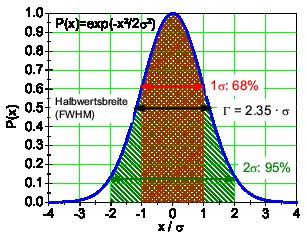
\includegraphics[width=8cm]{00_einl/gaussfkt}
% \end{captionbeside}
 \caption[Gau"ssche Glockenkurve]{\label{a:glockenkurve}Schematische Darstellung
   der Glockenkurve. Die Abzisse ist in Vielfachen von $\sigma$ angegeben.
   Auf die Normierung
   der Ordinate wurde der "Ubersicht wegen verzichtet. Die schraffierten
   Intervalle geben die jeweiligen Sicherheitsintervalle von 68.3~\%
   ($1\sigma$) und 95~\% ($2\sigma$) wieder (siehe Text).}
\end{figure}
%
Weiter kann folgende Formel hergeleitet werden:
%
\begin{equation} \label{i}
 s^2 = \int_{-\infty}^{+\infty}\,P(x) \cdot (x-\bar{x})^{2} dx = \sigma^{2}
\end{equation}
%
Das bedeutet, dass der Parameter $\sigma$ der Glockenkurve mit deren 
Standardabweichung $s$ "ubereinstimmt. Man kann
ferner zeigen, dass die Wahrscheinlichkeit, den wahren Wert
innerhalb des $1\sigma$"=Intervalls um $\bar{x}$ zu finden

\begin{equation} \label{j}
  W(\sigma) = \int_{\bar{x}-\sigma}^{\bar{x}+\sigma} \, P(x) dx =
  0.68
\end{equation}
%
betr"agt. Beziehung (\ref{j}) beinhaltet, dass die Angabe des
mittleren quadratischen Fehlers nicht bedeutet, dass f"ur alle
Messwerte $M_i$ die Abweichung vom Bestwert $M_B$ kleiner als
$\sigma$ ist. Vielmehr betr"agt die relative H"aufigkeit
(Wahrscheinlichkeit oder Sicherheit) hierf"ur nur 68\%.


\subsection{Der Bestwert einer Funktion und Fehlerfortpflanzung}

Der Bestwert einer Funktion $f(x,y,...)$ von verschiedenen
unabh"angigen Messgr"o"sen $x,y,...$ erschwert die Fehlerrechnung
etwas, und es muss das
Fehlerfortpflanzungsgesetz\index{Fehlerfortpflanzungsgesetz}
angewandt werden. Gegeben seien die Messwerte
%
\begin{equation} \label{l}
  x_{i},\quad i=1\ldots r; \hspace{2cm} y_{k},\quad k=1\ldots s \,
  ,
\end{equation}
%
aus denen ein Endergebnis $f_{i,k}=f(x_{i},y_{k})$ berechnet wird.
Beispiel: Berechnung der Fl"ache $A$ eines Rechtecks aus den
Kantenl"angen $x$ und $y$. Es l"asst sich zeigen, dass der Bestwert
$\bar A$ von $A$ gegeben ist durch
%
\begin{equation} \label{m}
 \bar f \equiv  \frac{1}{r} \cdot \frac{1}{s} \cdot
  \sum_{i=1}^{r} \sum_{k=1}^{s} f(x_{i},y_{k}) = f(\bar x, \bar y)
  \, .
\end{equation}
%
Dieses Ergebnis gilt f"ur beliebige Funktionen und beliebig viele
Variablen. Wir bezeichnen jetzt die mittleren quadratischen Fehler
von $f$, $x$ und $y$ mit $\sigma_f$, $\sigma_x$ bzw. $\sigma_y$.
Dann l"asst sich unter Benutzung der Definitionen der mittleren
quadratischen Fehler dieser drei Gr"o"sen zeigen, dass ein
Fehlerfortpflanzungsgesetz\index{Fehlerfortpflanzung} in der Form
%
\begin{equation} \label{n}
 \sigma_{f} =
   \sqrt{\sigma_{x}^{2} \left( \frac{\partial f}{\partial x} \right)^{2}
    +
         \sigma_{y}^{2} \left( \frac{\partial f}{\partial y} \right)^{2}
   }
\end{equation}
%
gilt\footnote{Die gilt, wie eingangs angenommen, {\it nur} f"ur unab"angige
Messgr"o"sen. Andernfalls muss ein zus"atzlicher Term, der die Korrelation
zwischen $x$ und $y$ ber"ucksichtig, hinzugef"ugt werden.}. 
Auch in (\ref{n}) sind beliebig viele Variablen zugelassen.
Spezialf"alle von (\ref{n}) sind:
%
\begin{equation} \label{o}
  \bar f = \bar x + \bar y \qquad \mbox{mit: } \qquad
  \sigma_{f} = \sqrt{\sigma_{x}^{2} + \sigma_{y}^{2}}
\end{equation}
%
\begin{equation} \label{q}
  \bar f = \bar x \cdot \bar y \qquad \mbox{mit: } \qquad
  \frac{\sigma_{f}}{\bar f}  = \sqrt{\left(\frac{\sigma_{x}}{\bar
 x}\right)^{2} + \left(\frac{\sigma_{y}}{\bar y}\right)^{2}} \, .
\end{equation}
%
%


\subsection{Der mittlere quadratische Fehler des Bestwertes}

Die Beziehung (\ref{f}) gibt den mittleren quadratischen Fehler
$\Delta M_{i}$ der Einzelmessung $M_{i}$ an.\footnote{Hier werden
h"aufig auch die Begriffe "`Standardabweichung"' $s$ oder
"`Varianz"' $s^2$ verwendet. Die Verwendung der Begriffe erfolgt
nicht immer einheitlich, man sollte daher auf die jeweilige
Definition achten.} Da aber nicht die Einzelmessung sondern der
Bestwert $M_B$ das Endergebnis darstellt, muss der Fehler des
Bestwertes\index{Fehler!des Mittelwertes} $\Delta M_{B}$ bestimmt
werden. Dazu fassen wir $M_B$ als Funktion der Gr"o"sen $M_{i}$ auf,
d.h.:
%
\begin{equation} \label{s}
M_{B} = \frac{1}{n} \sum_{i=1}^{n}\,M_{i} = f(M_{1}, M_{2},...)
\end{equation}
%
und wenden hierauf das Fehlerfortpflanzungsgesetz
%
\begin{equation} \label{t}
 \Delta M_{B} = \sqrt{\sum_{i=1}^{n}\,\left(\sigma_{i}\,\frac{\partial
 f}{\partial M_{i}}\right)^{2}}
\end{equation}
%
an. Da alle $\sigma_i$ als gleich angenommen werden k"onnen , d.h.
$\sigma_i$ =$\sigma$, und
%
\begin{equation} \label{u}
 \frac{\partial f}{\partial M_{i}} = \frac{1}{n}
\end{equation}
%
ist, ergibt sich schlie"slich:
%
\begin{important}
\begin{equation} \label{v}
 \Delta M_{B} = \frac{\sigma}{\sqrt{n}}  =
  \sqrt{\frac{1}{n(n-1)} \sum_{i=1}^{n} (\Delta M_{i})^{2}} \, .
\end{equation}
\end{important}
%
Genau dies sollte auch in den Protokollen zur Fehlerangabe
verwendet werden.




\subsection{Methode der kleinsten Fehlerquadrate (Minimales $\chi^2$)}

Ein h"aufig vorkommendes Problem ist die Anpassung einer glatten
Kurve an eine Folge von Messpunkten, die zur Bestimmung der
Kurvenparameter dienen sollen. Die Anpassung von Funktionen an
Messwerte erfolgt meist nach der Methode der kleinsten Quadrate
(minimales $\chi^2$). Als Beispiel benutzen wir das radioaktive
Zerfallsgesetz:
%
\begin{equation} \label{w}
  N(t)\,=\,N_{0} \exp(-\lambda t) \, ,
\end{equation}
%
welches die Anzahl $N(t)$ der nicht zerfallenen
radioaktiven Kerne als Funktion der Zeit $t$ beschreibt. In
(\ref{w}) ist $N_0$ die Zahl der Kerne zum Zeitpunkt $t=0$ und
$\lambda$ die Zerfallskonstante, die "uber die Beziehung
%
\begin{equation} \label{x}
  \lambda = \frac{\ln 2}{T_{1/2}}
\end{equation}
%
mit der Halbwertszeit $T_{1/2}$ des radioaktiven Materials
(Nuklids) zusammenh"angt. Zur Vereinfachung setzen wir voraus, dass
$N_0$ aus anderen Messungen bekannt ist, so dass nur noch
$T_{1/2}$ zu bestimmen ist. Wir messen $n$ mal die pro Zeiteinheit
stattfindenen Zerf"alle (Aktivit"at) und stellen uns die Aufgabe,
$T_{1/2}$ durch geeignete Anpassung der Funktion~(\ref{w}) an die
Messwerte zu bestimmen. Die Messung liefert
%
\begin{equation} \label{y}
 \mbox{Wertepaare} (N_i, t_i) \, ,
\end{equation}
%
d.h. die zum Zeitpunkt $t_i$ pro Zeiteinheit gemessene Anzahl
$N_i$ radioaktiver Kerne. Die Vorschrift f"ur die Anpassung der
Funktion (\ref{w}) lautet:
%
\begin{equation} \label{z}
  \chi^{2}(T_{1/2}) =
    \sum_{i=1}^{n} \frac{(N_{i}-N(t_{i}))^{2}}{\sigma_{i}^{2}} = \mbox{Minimum} \, .
\end{equation}
%
In (\ref{z}) bedeutet $\sigma_i$ den mittleren quadratischen
Fehler von $N_i$, der nach den Gesetzen der Statistik f"ur
diskrete, z"ahlbare Ereignisse
(Poisson-Statistik\index{Poisson-Statistik}) durch die Beziehung
%
\begin{equation} \label{aa}
  \sigma_i^2 = N_i
\end{equation}
%
gegeben ist. Wir vergleichen in (\ref{z}) also die Abweichung jedes
Messwertes $N_i$ von der gew"ahlten Kurve mit dem Fehler des
Messwertes und minimieren die Summe der mit dem reziproken Fehler
gewichteten Abweichungsquadrate\index{Abweichungsquadrate}.
Ausdr"ucke der Form (\ref{z}) werden allgemein mit $\chi^2$
bezeichnet und beinhalten die Gau"ssche Methode der kleinsten
Quadrate. Die praktische Auswertung der Vorschrift (\ref{z})
erfolgt, indem man $\chi^2$ f"ur eine Anzahl geeignet erscheinender
Werte $T_{1/2}$ berechnet und das Minimum mit Hilfe einer grafischen
Darstellung der Funktion $\chi^2$($T_{1/2}$) bestimmt.
%%%%%%%%%%%%%%%%%%%%%%%%%%%%%%%%%%%%%%%%%%%%%%%%%%%%%%%%%%%%%%%%%%%

\chapter {Erstellung von Diagrammen} \label{v:diagramme}

Hier folgen einige kurze Hinweise zur Erstellung von Diagrammen in
den Protokollen des Praktikums.

\section{Allgemeines}

Die meisten Auswertungen in der Physik werden heute mit sehr
umfangreichen Programmpaketen durchgef"uhrt, die auch gleichzeitig
eine komfortable Diagrammerstellung erlauben. Dennoch kann es
vorkommen, dass man eine einfache Auswertung sehr viel schneller
und mit guter Genauigkeit auch auf konventionellem Wege auf
Millimeterpapier oder Logarithmenpapier ausf"uhren kann. Zudem sind
die hier folgenden Hinweise auch sehr n"utzlich, wenn man
Computerprogramme zur Diagrammerstellung verwendet.

Manuelle Diagramme sind grunds"atzlich immer auf Millimeter- oder
Logarithmenpapier anzufertigen. Bei Computerprogrammen kann auf dies
verzichtet werden, dennoch sollte man auch hier auf eine leichte
Ablesbarkeit der Daten achten.

\section{Achsen}


\begin{enumerate}
    \item Wahl der Achsen: Die unabh"angige (die eingestellte)
    Variable sollte auf der waagerechten Achse, der "`x-Achse"'
    (Abszisse\index{Abszisse}), aufgetragen werden. Die abh"angige (die
    gemessene) Variable sollte auf der vertikalen Achse, der "`y-Achse"'
    (Ordinate\index{Ordinate}), aufgetragen werden.
    \item Achseneinteilung: Die Achseneinteilung sollte so gew"ahlt
    werden, das die Werte eines Datenpunktes einfach und schnell
    ermittelt werden k"onnen. Drei Einheiten einer Gr"o{\ss}e auf einem Zentimeter einzuzeichnen macht also nicht viel Sinn.
    \item Nullpunktsunterdr"uckung: Der Wertebereich der Achsen
    sollte so gew"ahlt werden, dass ein m"oglichst gro"ser Bereich
    ausgef"ullt wird (mindestens 75\% des Diagrammbereiches). Hierbei kann der Nullpunkt
    unterdr"uckt werden, wenn kein triftiger Grund dagegen
    spricht. Das bedeutet, dass die Einheiten auf Abszisse und Ordinate nicht unbedingt bei x=y=0 anfangen m"ussen. Dies gilt auch f"ur logarithmische Skalen.
    \item Achsen sind zu beschriften! Was ist aufgetragen?
    Zahlenwerte sind anzugeben. Einheiten sind unverzichtbar.
    \item Bei logarithmierten Werten ist die Angabe der Einheit problematisch,
     da der Logarithmus im Argument keine Einheit haben darf. Hier teilt man die
     Messwerte einfach durch die Einheit und erh"alt so reine Zahlenwert. Dies ist
     dann auch so anzugeben.
\end{enumerate}

\section{Datenpunkte und Fehlerbalken}

\begin{itemize}
    \item Symbole: Die Messpunkte sollten durch deutliche Symbole
    gekennzeichnet werden. "Ublich sind zum Beispiel: $ \square \blacksquare
    \blacktriangle \blacktriangledown \lozenge \blacklozenge \vartriangle
    \triangledown \bullet \bigcirc \circ \ast \star$.
    \item Unterschiedliche Messreihen sollten auch durch
    unterschiedliche Symbole gekennzeichnet werden. Auf eine
    eindeutige Legende ist zu achten. Farbe kann hier sehr
    n"utzlich sein, doch diese geht leider beim Kopieren verloren.
    \item Fehlerbalken: Normalerweise sind alle Messpunkte mit
    Fehlerbalken zu versehen, deren L"ange der Gr"o"se des (1$\sigma$-)Fehlers
    auf den jeweiligen Messwert entspricht. Dabei kann es notwendig sein, in
    den verschiedenen Achsrichtungen unterschiedlich gro"se
    Fehlerbalken zu verwenden.
\end{itemize}

\section{Kurven und Verbindungslinien}


\begin{itemize}
    \item Eine durchgezogene Kurve kann die Lesbarkeit einer
    Darstellung deutlich erh"ohen. Dennoch sollte dies mit Bedacht
    angewendet werden.
    \item In allen F"allen des Praktikums sind "`glatte"' Kurven zu
    erwarten. Zumeist ist der funktionale Zusammenhang der
    Messdaten auch durch die Theorie schon bekannt. Im Allgemeinen
    sollte eine Kurve m"oglichst wenig Wendepunkte haben.
    \item Es ist nicht zwingend erforderlich, dass die
    durchgezogene Kurve alle, oder "uberhaupt, Messpunkte trifft.
    Endpunkte sind meist weniger genau und m"ussen nicht unbedingt
    getroffen werden. Das einfache lineare Verbinden der
    Messpunkte durch eine
    "`Zick-Zack-Kurve"' ist physikalisch kompletter Unsinn und
    sollte unterlassen werden.
    \item Die Kurve sollte m"oglichst dicht an den Messpunkten
    liegen (Minimierung der Fehlerquadrate). Die eingezeichneten
    Fehlerbalken k"onnen hier eine gute Hilfe sein. Zudem ist das
    Auge ein sehr guter "`Computer"' f"ur die Ausgleichskurve.
    \item Im Wesentlichen sollte die Kurve die Messpunkte
    halbieren, d.h. eine H"alfte der Punkte "uber der Kurve, die
    andere darunter. Das gilt sinngem"a"s auch f"ur Teilst"ucke.
    \item An Regressionsgeraden sind auch die Ergebnisse der
    Regression mit den richtigen Einheiten anzugeben.
    \item Bei Ermittlung des Fehlers "uber Grenzgeraden, sind auch
    diese in der Zeichnung anzudeuten.
\end{itemize}

Als Beispiel f"ur die Diagrammerstellung sind in
Bild~\ref{a:graph_beisp} zwei typische Diagramme aufgef"uhrt.
%
\begin{figure}[htb]
  \centering
  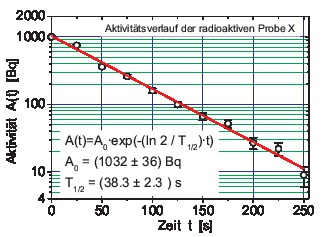
\includegraphics[width=6.5cm]{00_einl/graph_expzerf}
  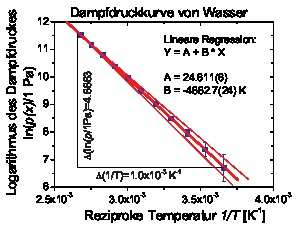
\includegraphics[width=6.5cm]{00_einl/graph_dampf}
  \caption[Diagramm-Beispiele]{\label{a:graph_beisp}Beispiele f"ur grafische Auftragungen
   zu Messwerten und Auswertungen:
  a) (links) Halblogarithmische Darstellung des exponentiellen Zerfalls;
  b) (rechts) Arrheniusplot der Dampfdruckkurve von Wasser. }
\end{figure}
%
Die Aktivit"atskurve wird
halblogarithmisch\index{Logarithmenpapier!halblogarithmisch}
aufgetragen, d.h. die Zeit normal (linear) als x-Achse, w"ahrend
die Aktivit"at logarithmisch
(Logarithmenpapier\index{Logarithmenpapier}) aufgetragen
wird.\footnote{Es erfolgt keine Umrechnung der Messwerte, die
Skalenteilung ist logarithmisch, genauer gesagt
halblogarithmisch.} Dies hat zur Folge, dass aus der
Exponentialfunktion eine lineare Funktion wird:
%
\begin{equation}\label{e:bsp_exp}
    A(t)=A_0 \cdot \exp(-\lambda t) \Longrightarrow \ln(A(t)) =
    \ln(A_0) - \lambda t
\end{equation}
%
Die Zerfallskonstante $\lambda$ kann dann aus der Steigung $m$ der
sich ergebenden Geraden ermittelt werden, woraus dann die
Halbwertszeit folgt. Man beachte die unterschiedliche L"ange der
Fehlerbalken. F"ur viele Skalengesetze und stark streuende Messwerte,
oder wenn man den Zusammenhang nicht genau kennt, verwendet man die
doppeltlogarithmische
Auftragung\index{Logarithmenpapier!doppeltlogarithmisch}, die f"ur
fast alle beliebigen Messungen eine Gerade entstehen l"asst.

In Bild~\ref{a:graph_beisp}b) ist ein Arrheniusplot des Dampfdruckes
von Wasser aufgetragen. Hier werden die Messwerte (in Pa) vor dem
Auftragen durch ihren Logarithmus ersetzt. Da das Argument des
Logarithmus keine Einheit enthalten kann, behilft man sich, indem
man durch die Einheit dividiert (d.h. diese "`Basiseinheit"' muss
auch im Diagramm mit angegeben werden). Durch die Auftragung der
logarithmierten Messwerte gegen die reziproke Temperatur erh"alt man
eine Gerade
%
\begin{equation}\label{e:bsp_dampf}
    p(T) = p_0 \cdot \exp\left( - \frac{\Lambda}{RT} \right) \Rightarrow
    \ln\left( p(T) \right) = \ln(p_0) - \frac{\Lambda}{R} \cdot
    \frac{1}{T} \, ,
\end{equation}
%
aus deren Steigung die Verdampfungsenthalpie $\Lambda$ berechnet
werden kann. Das Steigungsdreieck ist eingezeichnet und die Steigung
ergibt sich zu
$m=\frac{\mathrm{4.883}}{\mathrm{1\cdot 10^{-3}\, K^{-1}}}=\mathrm{4883~K}$.\footnote{Bitte
beachten Sie, dass die Steigung nat"urlich eine Einheit hat, die
angegeben werden muss.} Mit der allgemeinen Gaskonstanten
$R=\mathrm{8.3145\,J \, mol^{-1} \, K^{-1}}$ ergibt sich die
Verdampfungsw"arme zu $\Lambda=m \cdot R = \mathrm{40597\,J \,mol^{-1}}$ mit einem Fehler von $\Delta \Lambda = \mathrm{20\,J \,mol^{-1}}$.

%%%%%%%%%%%%%%%%%%%%%%%%%%%%%%%%%%%%%%%%%%%%%%%%%%%%%%%%%%%%%%%%%%%

\chapter{Verzeichnis der Versuche}

\begin{table}[h!]
 \centering
 \begin{tabular}{rll}
 \hline
 Versuch & Thema & Raum\\
 \hline
 1 & Solarzelle und Halbleiterdiode & A.02.106\\ 
 2 & Stoß & A.02.105\\
 3 & Wechselstrom und R-C-Kreis & A.01.108 \\ 
 4 & Spule und Transformator & A.01.108 \\ 
 5 & Pohl'scher Resonator & A.02.104 \\
 6 & Trägheitsmoment & A.02.105\\
 7 & Kapillarität und Auftrieb & A.02.102 \\ 
 8 & Innere Reibung von Flüssigkeiten & A.02.102 \\ 
 9 & Linsengesetze & A.01.104 \\ 
 10 & Mikroskop & A.02.107 \\ 
 11 & Brechungsindex von Glas & A.02.108 \\ 
 12 & Beugung am Gitter & A.02.108\\ 
 13 & Thermoelement & A.01.102 \\ 
 14 & Ultraschall & A.01.116\\
 15 & Signalausbreitung auf Leitern & A.01.117 \\ 
 16 & Diffusion & A.01.102\\ 
 17 & Künstliche Radioaktivität & A.01.116 \\ 
 18 & Spezifische Elektronenladung & A.01.105 \\ 
 19 & Spezifische Wärmekapazität & A.02.102 \\ 
 20 & Spezifische Wärmekapazität von Luft & A.01.102 \\ 
 \hline
 \end{tabular}
\end{table}
  
%
%%%%%%%%%%%%%%%%%%%%%%%%%%%%%%%%%%%%%%%%%%%%%%%%%%%%%%%%%%%%%%%%%%%%
\cleardoublepage
\part{Versuche}


\renewcommand{\thechapter}{\arabic{chapter}}
\setcounter{chapter}{0}
\def\chaptername{Versuch}
\setcounter{tocdepth}{0}
%
%%%%%%% Vorf�hrversuch %%%%%%%
\import{Versuch_0/}{Anleitung-0}
%%%%%%%%%%%%%%%%%%%%%%%%%%%%%%
%
\import{Versuch_1-2n/}{Anleitung-1}	% Solarzelle und Hlableiterdiode
\import{Versuch_1-2n/}{Anleitung-2}			% Sto�

\import{Versuch_3-4n/}{Anleitung-3}	% Wechselstrom und RC Kreis
\import{Versuch_3-4n/}{Anleitung-4}	% Spule und Transformator

\import{Versuch_5-6n/}{Anleitung-5}	% Pohl'scher Resonator
\import{Versuch_5-6n/}{Anleitung-6}			% Drehschwingungen --> Tr�gheitsmoment

\import{Versuch_7-8n/}{Anleitung-7}			% Kapillarit�t und Auftrieb
\import{Versuch_7-8n/}{Anleitung-8}			% Innere Reibung von Fl�ssigkeiten

\import{Versuch_9-10n/}{Anleitung-9}			% Linsengesetze
\import{Versuch_9-10n/}{Anleitung-10}			% Mikroskop

\import{Versuch_11-12n/}{Anleitung-11}		% Brechungsindex von Glas
\import{Versuch_11-12n/}{Anleitung-12}		% Beugung am Gitter

\import{Versuch_13-14n/}{Anleitung-13}	% Thermoelement
\import{Versuch_13-14n/}{Anleitung-14}	% Ultraschall

\import{Versuch_15-16n/}{Anleitung-15}	% Elektrische Netzwerke
\import{Versuch_15-16n/}{Anleitung-16} 	% Nichtstation�re Diffusion

\import{Versuch_17-18n/}{Anleitung-17}	% K�nstliche Radioaktivit�t
\import{Versuch_17-18n/}{Anleitung-18}	% Spezifische Elektronenladung e/m

\import{Versuch_19-20n/}{Anleitung-19}			% Spezifische W�rmekapazit�t
\import{Versuch_19-20n/}{Anleitung-20}			% Molare W�rmekapazit�t von Luft

%%%%%%%%%%%%%%%%%%%%%%%%%%%%%%%%%%%%%%%%%%%%%%%%%%%%%%%%%%%
%
%\cleardoublepage
%\appendix
%%
%%%%%%%%%%%%%%%%%%%%%%%%%%%%%%%%%%%%%%%%%%%%%%%%%%%%%%%%%%%%
%
\backmatter

\renewcommand{\thechapter}{\Roman{chapter}}
\setcounter{chapter}{10}

 \include{00_einl/raumverz}

\end{document}

